% mnras_template.tex
%
% LaTeX template for creating an MNRAS paper
%
% v3.3 released April 2024
% (version numbers match those of mnras.cls)
%
% Copyright (C) Royal Astronomical Society 2015
% Authors:
% Keith T. Smith (Royal Astronomical Society)

% Change log
%
% v3.3 April 2024
%   Updated \pubyear to print the current year automatically
% v3.2 July 2023
%	Updated guidance on use of amssymb package
% v3.0 May 2015
%    Renamed to match the new package name
%    Version number matches mnras.cls
%    A few minor tweaks to wording
% v1.0 September 2013
%    Beta testing only - never publicly released
%    First version: a simple (ish) template for creating an MNRAS paper

%%%%%%%%%%%%%%%%%%%%%%%%%%%%%%%%%%%%%%%%%%%%%%%%%%
% Basic setup. Most papers should leave these options alone.
\documentclass[fleqn,usenatbib]{mnras}

% MNRAS is set in Times font. If you don't have this installed (most LaTeX
% installations will be fine) or prefer the old Computer Modern fonts, comment
% out the following line
\usepackage{newtxtext,newtxmath}
\usepackage[T1]{fontenc}
\usepackage{graphicx}
\usepackage{amsmath}
\usepackage{booktabs}
\usepackage{xcolor}
\usepackage[normalem]{ulem}
\usepackage{cancel}

\newcommand{\dd}{\mathrm{d}}
\newcommand{\ee}{\mathrm{e}}
\newcommand{\bs}[1]{\boldsymbol{#1}}
\newcommand{\avg}[1]{\left\langle #1 \right\rangle}
\newcommand{\Cov}{\operatorname{Cov}}
\newcommand{\xminus}{\bs{x}_{-}}
\newcommand{\xplus}{\bs{x}_{+}}
\newcommand{\revadd}[1]{\textcolor{red}{#1}}
\newcommand{\revdel}[1]{\textcolor{red}{\sout{#1}}\hspace{0.18em}}
\newcommand{\revaddmath}[1]{\textcolor{red}{#1}}
\newcommand{\revdelmath}[1]{\textcolor{red}{\cancel{#1}}}

% Depending on your LaTeX fonts installation, you might get better results with one of these:
%\usepackage{mathptmx}
%\usepackage{txfonts}

% Allow "Thomas van Noord" and "Simon de Laguarde" and alike to be sorted by "N" and "L" etc. in the bibliography.
% Write the name in the bibliography as "\VAN{Noord}{Van}{van} Noord, Thomas"
\DeclareRobustCommand{\VAN}[3]{#2}
\let\VANthebibliography\thebibliography
\def\thebibliography{\DeclareRobustCommand{\VAN}[3]{##3}\VANthebibliography}


%%%%% AUTHORS - PLACE YOUR OWN COMMANDS HERE %%%%%

% Please keep new commands to a minimum, and use \newcommand not \def to avoid
% overwriting existing commands. Example:
%\newcommand{\pcm}{\,cm$^{-2}$}	% per cm-squared

\newcommand{\slug}{\textsc{slug}}
%\defcitealias{Zhang2025}{Paper I}
\defcitealias{KT18}{Paper I}
\defcitealias{KT25}{Paper II}
\defcitealias{RoSE}{RoSE}

% Autoref macros
\def\sectionautorefname{Section}
\def\subsectionautorefname{Section}
\def\subsubsectionautorefname{Section}
\def\figureautorefname{Figure}
\def\tableautorefname{Table}
\def\equationautorefname{equation}
\newcommand{\aref}[1]{\hyperref[#1]{Appendix~\ref{#1}}}
%%%%%%%%%%%%%%%%%%%%%%%%%%%%%%%%%%%%%%%%%%%%%%%%%%

% for orcid
\usepackage{scalerel,tikz}
\usetikzlibrary{svg.path}
\definecolor{orcidlogocol}{HTML}{A6CE39}
\tikzset{orcidlogo/.pic={
\fill[orcidlogocol] svg{M256,128c0,70.7-57.3,128-128,128C57.3,256,0,198.7,0,128C0,57.3,57.3,0,128,0C198.7,0,256,57.3,256,128z};
\fill[white] svg{M86.3,186.2H70.9V79.1h15.4v48.4V186.2z}
svg{M108.9,79.1h41.6c39.6,0,57,28.3,57,53.6c0,27.5-21.5,53.6-56.8,53.6h-41.8V79.1z M124.3,172.4h24.5c34.9,0,42.9-26.5,42.9-39.7c0-21.5-13.7-39.7-43.7-39.7h-23.7V172.4z}
svg{M88.7,56.8c0,5.5-4.5,10.1-10.1,10.1c-5.6,0-10.1-4.6-10.1-10.1c0-5.6,4.5-10.1,10.1-10.1C84.2,46.7,88.7,51.3,88.7,56.8z};
}}
\newcommand\orcidicon[1]{\href{https://orcid.org/#1}{\mbox{\scalerel*{

\begin{tikzpicture}[yscale=-1,transform shape]
\pic{orcidlogo};
\end{tikzpicture}
}{|}}}}

%%%%%%%%%%%%%%%%%%% TITLE PAGE %%%%%%%%%%%%%%%%%%%

% Title of the paper, and the short title which is used in the headers.
% Keep the title short and informative.
\title[KTZ in PHANGS--MUSE galaxies]{Metallicity fluctuation statistics in the interstellar medium and young stars -- IV. A PHANGS--MUSE application of non-uniform injection}

% The list of authors, and the short list which is used in the headers.
% If you need two or more lines of authors, add an extra line using \newauthor
\author[C. Zhang et al.]{\ignorespaces
Chuhan Zhang$^{\orcidicon{0009-0000-2503-4803}{1}}$\thanks{E-mail: chuhan.zhang@anu.edu.au},
Mark R. Krumholz$^{\orcidicon{0000-0003-3893-854X}{1}}$,
Yuan-Sen Ting$^{\orcidicon{0000-0001-5082-9536}{2,3}}$
\\
% List of institutions
$^{1}$Research School of Astronomy and Astrophysics, Australian National University, Cotter Road, Weston ACT 2611, Australia\\
$^{2}$Department of Astronomy, The Ohio State University, Columbus, OH 43210, USA\\
$^{3}$Max-Planck-Institut f\"ur Astronomie, K\"onigstuhl 17, D-69117 Heidelberg, Germany\\
}


% These dates will be filled out by the publisher
\date{Accepted XXX. Received YYY; in original form ZZZ}

% Prints the current year, for the copyright statements etc. To achieve a fixed year, replace the expression with a number. 
\pubyear{\the\year{}}

\begin{document}
\label{firstpage}
\pagerange{\pageref{firstpage}--\pageref{lastpage}}
\maketitle

\begin{abstract}
We apply the non-uniform KTZ metal-correlation model developed in the companion theory paper to four nearby spiral galaxies observed by PHANGS--MUSE: NGC~628, NGC~1566, NGC~4254, and NGC~4303.  Emission-line maps are matched to a 120-pc point-spread function, sampled on a 60-pc face-on grid, and converted to oxygen-abundance residuals after line-quality, star-forming BPT, equivalent-width, and coverage selections.  Missing cells remain absent from the exhaustive finite-window pair statistic, and the same footprint, radial-profile subtraction, beam response, and selection covariance are propagated through KTZ and KT18.  We compare three source geometries specified without using the metallicity residuals: a 1-kpc-smoothed two-dimensional H$\alpha$ intensity template, the released PHANGS arm-region mask, and a continuous H$\alpha$ harmonic model.  The complete KTZ likelihood contains the conditionally Poisson same-event and deterministic mean-field terms together with the isotropic distinct-event term $C_{\rm NP}$ derived in the theory paper.  The comparison is an exploratory test of sensitivity to source morphology and observing transfer, rather than a detection of phase-locked chemical structure.  It demonstrates how KTZ can be confronted with resolved maps while identifying source geometry, selection, covariance calibration, and the approximate projection of a non-axisymmetric covariance as the limiting systematics.
\end{abstract}

\begin{keywords}
galaxies: abundances -- galaxies: ISM -- galaxies: spiral -- ISM: abundances -- methods: data analysis
\end{keywords}

\section{Introduction}
\label{sec:intro}

Spatially resolved metallicity fluctuations contain information that is absent from a radial abundance gradient.  Localised enrichment, turbulent transport, and the organisation of star formation determine both the amplitude and the coherence scale of residual abundance structure.  Integral-field spectroscopy now permits these residuals to be mapped across nearby galaxies, and two-point statistics show that chemically coherent structure commonly persists over hundreds of parsecs to kiloparsec scales \citep[e.g.,][]{2020MNRAS.499..193K,Li2021,2021MNRAS.508..489M,2023MNRAS.518..286L}.

The uniform stochastic-injection theory of \citet[hereafter \citetalias{KT18}]{KT18} connects the correlation function to injection width, diffusion, and the duration over which enrichment events accumulate.  Its multi-element extension, \citet[hereafter \citetalias{KT25}]{KT25}, adds channel-dependent yields, delays, and stellar drift.  These models provide physically interpretable baselines, but a uniform source process cannot retain the phase of a spiral pattern or distinguish a coherent arm-associated mean field from residual association-scale clustering.  Those limitations are especially relevant when observed correlations contain intermediate-scale shoulders or cross zero at large separation.

The companion theory paper in this series (Paper III) develops KTZ, an extension in which the deterministic injection intensity follows an externally specified two-dimensional source template.  It separates the same-event covariance, its local rate modulation, the product of any unremoved non-axisymmetric mean field, and the connected covariance between distinct events.  Paper III also derives finite-window and multi-element statistics and validates them against controlled Monte Carlo experiments.  Here we ask how that decomposition can be implemented on real maps once the beam, incomplete footprint, abundance selection, radial-profile subtraction, and correlated measurement errors are included.

We analyse NGC~628, NGC~1566, NGC~4254, and NGC~4303 using public PHANGS--MUSE emission-line products and source geometries specified independently of the metallicity residuals.  The aims are to implement the pair-product statistic on realistic maps, compare a direct two-dimensional H$\alpha$ source field with pixel-domain arm regions and an analytic harmonic compression, and determine how strongly the inferred transport and residual source-pair coordinates depend on that choice.  Because these galaxies and alternative geometries have already been inspected during method development, the resulting comparisons are exploratory rather than a pre-registered population test.

\autoref{sec:framework} summarises the KTZ quantities used in the likelihood.  \autoref{sec:application} describes the public data, map construction, observing transfer, and inference.  \autoref{sec:discussion} interprets the current four-galaxy geometry comparison and delineates which conclusions are supported by the derived theory.

\section{KTZ framework for resolved maps}
\label{sec:framework}

Paper III considers enrichment events with initial Gaussian width $\sigma$, diffusion coefficient $\kappa$, and maximum source age $t_\ast$.  The transport scale, relative injection width, and relative deterministic-mean strength used below are
\begin{align}
    \ell_\ast&=\sqrt{\sigma^2+2\kappa t_\ast},
    &\epsilon&=\frac{\sigma}{\ell_\ast},
    \label{eq:dimensionless_variables}
    \\
    \beta_{\rm src}
    &=\frac{4\pi\kappa\lambda_0t_\ast^2\langle M_\ast\rangle^2}
    {\langle M_\ast^2\rangle}.
    \label{eq:beta_src}
\end{align}
Here $\lambda_0$ is the local axisymmetric event rate and $M_\ast$ is the stellar mass represented by one parent event.  For a source harmonic of order $n$, the dimensionless smoothing coordinate is $q_n=nk_\perp\ell_\ast$.  The quantity $\beta_{\rm src}$ measures the deterministic mean-field power relative to the same-event second moment.

Let $\bs{x}_\pm=\bs{x}_m\pm\bs r/2$ be the two endpoints.  After subtraction of the axisymmetric abundance profile, the complete KTZ model writes the residual second moment as
\begin{equation}
    C_{\rm obs}(\bs{x}_-,\bs{x}_+)
    =C_{{\rm 2p},0}+C_{{\rm 2p},N}+C_{\rm M}+C_{\rm NP}.
    \label{eq:ktz_component_summary}
\end{equation}
The first two terms are the uniform and source-modulated parts of the connected same-event covariance.  The third is the product of the deterministic non-axisymmetric means left in the residual map and is therefore not a connected covariance about the full ensemble mean.  The fourth describes residual association between distinct events after the deterministic source intensity has been specified.  Following the notation and validated isotropic model of the theory paper, we denote this contribution simply by $C_{\rm NP}$, with Gaussian pair excess
\begin{equation}
    {\cal E}_{\rm src}(\Delta)
    ={\cal A}_{\rm src}
    \exp\left(-\frac{\Delta^2}{2\ell_{\rm src}^2}\right),
    \label{eq:Esrc_example}
\end{equation}
and propagate it through both age-integrated transport kernels.  Its local normalisation follows the squared axisymmetric rate $\lambda_0^2(R)$, but it is not multiplied by the non-axisymmetric source template.  Thus $C_{\rm NP}$ enters the numerator and endpoint second moments before normalisation; it is not an additive correction to a completed KTZ curve or an additional spiral harmonic.

Define $V_-=C_{\rm obs}(\bs{x}_-,\bs{x}_-)$ and $V_+=C_{\rm obs}(\bs{x}_+,\bs{x}_+)$.  If $\langle\cdot\rangle_3$ denotes an average over every allowed pair midpoint and orientation in a separation bin, the finite-window statistic is
\begin{equation}
    \xi_{3,{\rm pp}}(r)
    =\frac{\langle C_{\rm obs}\rangle_3(r)}
    {[\langle V_-\rangle_3(r)\langle V_+\rangle_3(r)]^{1/2}}.
    \label{eq:xi3_pp_def}
\end{equation}
The numerator and endpoint second moments must be averaged separately because averaging and normalisation do not commute.  The implementation below evaluates the Paper III kernels on the observed source template and applies the same finite footprint and map-processing operators used for the data.

\section{PHANGS--MUSE application}
\label{sec:application}

\subsection{Implementation on PHANGS--MUSE maps}
\label{ssec:phangs_implementation}

We now demonstrate how the finite-window statistic in equation~(\ref{eq:xi3_pp_def}) can be measured and fitted in resolved abundance maps.  We restrict this application to four nearby spiral galaxies observed by PHANGS--MUSE: NGC~628, NGC~1566, NGC~4254, and NGC~4303 \citep{2022A&A...659A.191E}.  In each case the public MUSE footprint covers a substantial fraction of the interval $0.1\leq R/R_{25}\leq0.4$, and the non-axisymmetric source geometry can be specified independently of the abundance field by the released PHANGS environment mask.  No other galaxy enters the analysis reported below.

\subsubsection{Public data and common physical grid}
\label{sssec:phangs_data}

For each galaxy we use five public PHANGS products: the PSF-homogenised (\texttt{copt}) emission-line MAPS file, the matched synthetic SDSS-$r$ image, the nebular catalogue, its segmentation mask, and the simple pixel-level environment mask of \citet{Querejeta2021} (data DOI 10.11570/21.0024).  The MAPS/SDSS-$r$ ESO product pairs are ADP.2021-07-16T10:20:56.338/.336 (NGC~628), .422/.420 (NGC~1566), .482/.480 (NGC~4254), and .494/.492 (NGC~4303).  The corresponding catalogue/mask pairs are ADP.2025-05-14T09:12:30.213/.214, .227/.228, .237/.238, and .239/.240, respectively.  The catalogue supplies the disc-coordinate transformation and an external calibration of the H$\alpha$ equivalent width; catalogue metallicities are not used to construct the abundance maps or their correlations.  The environment masks supply finite, pixel-domain arm footprints.  They are morphological classifications rather than H$\alpha$ segmentations: \citet{Querejeta2021} visually identify bright arm points in unsharp-masked Spitzer 3.6-$\mu\mathrm{m}$ images, fit each segment in logarithmic polar coordinates, adjust its azimuthal endpoints by eye, and assign a finite width from an empirical CO-flux convergence criterion.  The resulting arm regions are typically 1--2~kpc wide and intentionally accommodate tracer offsets, spurs, and local departures from an ideal logarithmic spiral.  The ``simple'' product then assigns each pixel to one mutually exclusive dominant environment.  The adopted geometry and resulting samples are listed in Table~\ref{tab:phangs_sample}.

Throughout this application, $R_{25}$ denotes the physical semi-major-axis radius of the $B$-band $\mu_B=25~\mathrm{mag~arcsec}^{-2}$ isophote; it is not remeasured from the MUSE mosaics.  We adopt the angular radii $\theta_{25}=4.9$, $3.6$, $2.5$, and $3.4$~arcmin for NGC~628, NGC~1566, NGC~4254, and NGC~4303, respectively.  These are the HyperLEDA values \citep{2014A&A...570A..13M} compiled for the PHANGS--MUSE sample \citep{2022A&A...659A.191E}.  For a distance $D$ in Mpc, the physical radii in Table~\ref{tab:phangs_sample} are calculated as
\begin{equation}
    R_{25}=10^3 D\tan\left(\frac{\pi\theta_{25}}{180\times60}\right)~\mathrm{kpc},
    \label{eq:phangs_r25_conversion}
\end{equation}
which is equivalent to the small-angle relation at these angular sizes.  Thus both the analysis interval $0.1\leq R/R_{25}\leq0.4$ and the conversion of the catalogue coordinate \texttt{DEPROJ\_R\_R25} to kpc use the same external optical-radius convention.

\begin{table*}
\centering
\caption{PHANGS--MUSE sample and fixed map geometry.  The listed $R_{25}$ values are the physical radii obtained from the HyperLEDA angular radii and the adopted distances.  The radial limits are $0.1R_{25}$ and $0.4R_{25}$, $\mathrm{FWHM}_{\rm nat}$ is the resolution of the public \texttt{copt} product, and $N_{\rm pix}$ is the number of 60-pc face-on cells that pass every abundance-map selection.}
\label{tab:phangs_sample}
\begin{tabular}{@{}lrrrrrrr@{}}
\toprule
Galaxy & $D$ [Mpc] & $R_{25}$ [kpc] & $i$ [deg] & PA [deg] & $\mathrm{FWHM}_{\rm nat}$ [arcsec] & $R$ [kpc] & $N_{\rm pix}$\\
\midrule
NGC~628  &  9.8 & 13.97 &  8.9 &  20.7 & 0.92 & 1.40--5.59 & 15,201\\
NGC~1566 & 17.7 & 18.54 & 29.5 & 214.7 & 0.80 & 1.85--7.41 & 27,451\\
NGC~4254 & 13.1 &  9.53 & 34.4 &  68.1 & 0.89 & 0.95--3.81 & 11,152\\
NGC~4303 & 17.0 & 16.81 & 23.5 & 312.4 & 0.78 & 1.68--6.73 & 33,708\\
\bottomrule
\end{tabular}
\end{table*}

We convolve the H$\beta$, [O~\textsc{iii}]~$\lambda5007$, H$\alpha$, [N~\textsc{ii}]~$\lambda6583$, and [S~\textsc{ii}]~$\lambda\lambda6717,6731$ surface-brightness and variance maps from their native \texttt{copt} resolution to a common circular Gaussian FWHM of 120~pc.  Convolution is performed before any line ratio is formed.  The maps are then sampled by bilinear interpolation on a 60-pc Cartesian grid in the face-on plane.  The sky-to-disc transformation is obtained by six iterations of an affine least-squares fit from catalogue sky coordinates to the released deprojected $(R,\phi)$ coordinates.  After each iteration, points with a positional residual exceeding the larger of 0.10~kpc and the median plus $10\times1.4826$ median absolute deviations are rejected.  The resulting single transformation is used for every line, the continuum map, and the environment mask.  A cell is retained only if at least 0.8 of the convolution kernel is supported by valid native pixels and every line listed above has $S/N\geq2$ after multiplying the released uncertainties by the fixed factor 1.12; this factor is part of the adopted measurement-error model and is not fitted.

We follow the resolved-map selection of \citet{Li2021}.  Let
\begin{equation}
    x_{\rm BPT}=\log_{10}\frac{[\mathrm{N\,II}]\lambda6583}{\mathrm{H}\alpha},
    \qquad
    y_{\rm BPT}=\log_{10}\frac{[\mathrm{O\,III}]\lambda5007}{\mathrm{H}\beta}.
\end{equation}
We retain cells with $x_{\rm BPT}<0.40$ and the theoretical maximum-starburst criterion \citep{Kewley2001}
\begin{equation}
    y_{\rm BPT}<\frac{0.61}{x_{\rm BPT}-0.47}+1.19,
\end{equation}
and require $\mathrm{EW}(\mathrm{H}\alpha)>6$~\AA.  Since the MAPS product has no continuum extension, the continuum density is taken from the matched synthetic SDSS-$r$ image.  For each galaxy, the multiplicative conversion between the gridded H$\alpha/r$ ratio and equivalent width is the median ratio to \texttt{EW\_HA6562\_FIT} over qualified catalogue regions, after a $5\times1.4826$ median-absolute-deviation clip in log space.  The segmentation mask is used only for this calibration, not to select abundance pixels; valid diffuse star-forming cells outside segmented nebulae are consequently retained.

Internal attenuation is corrected cell by cell with an intrinsic Balmer decrement of 2.86 and the $R_V=3.1$ O'Donnell optical curve \citep{ODonnell1994}.  Explicitly,
\begin{equation}
    \begin{aligned}
    E(B-V)&=
    \frac{2.5}{k(\mathrm{H}\beta)-k(\mathrm{H}\alpha)}
    \log_{10}\left[\frac{(\mathrm{H}\alpha/\mathrm{H}\beta)}{2.86}\right],\\
    F_{0,\lambda}&=F_\lambda 10^{0.4k(\lambda)E(B-V)}.
    \end{aligned}
    \label{eq:phangs_reddening}
\end{equation}
where $E(B-V)$ is clipped to $[0,2]$ to prevent noise fluctuations from implying negative attenuation or an unbounded correction.  Oxygen abundance is then calculated with the Pilyugin--Grebel $S$ calibration \citep{PilyuginGrebel2016}.  Defining the dereddened ratios
\begin{equation}
    \begin{aligned}
    R_3&=1.35\frac{[\mathrm{O\,III}]\lambda5007}{\mathrm{H}\beta},
    &N_2&=1.34\frac{[\mathrm{N\,II}]\lambda6583}{\mathrm{H}\beta},\\
    S_2&=\frac{[\mathrm{S\,II}]\lambda6717
    +[\mathrm{S\,II}]\lambda6731}{\mathrm{H}\beta}.
    \end{aligned}
\end{equation}
and $X=\log_{10}(R_3/S_2)$, $N=\log_{10}N_2$, and $S=\log_{10}S_2$, the implemented calibration for $Z_{\rm O}\equiv12+\log_{10}(\mathrm{O/H})$ is
\begin{equation}
  Z_{\rm O}=
  \begin{cases}
  \begin{aligned}
  &8.424+0.030X+0.751N\\[-2pt]
  &\quad+(-0.349+0.182X+0.508N)S,
  \end{aligned}
  &N\geq-0.6,\\[4pt]
  \begin{aligned}
  &8.072+0.789X+0.726N\\[-2pt]
  &\quad+(1.069-0.170X+0.022N)S,
  \end{aligned}
  &N<-0.6.
  \end{cases}
  \label{eq:phangs_scalibration}
\end{equation}
No additional cut on the derived abundance uncertainty is imposed.

To remove the axisymmetric abundance profile in the same manner as \citet{Li2021}, we subtract an independent arithmetic mean in every 0.2-kpc annulus containing at least 20 valid cells.  We finally subtract the arithmetic mean of all retained residuals, which changes the measured correlations by less than $1.1\times10^{-7}$ in these four maps.  Cells that fail any selection remain \texttt{NaN}; they are never assigned a zero abundance.  The upper row of Fig.~\ref{fig:phangs_four_galaxies} shows the precise residual fields entering the statistic.

The annular subtraction is a linear observing operation and must also be applied to the model.  If $a(i)$ is the 0.2-kpc annulus containing valid cell $i$, $n_a$ is the number of valid cells in annulus $a$, and $\mathbf P$ is defined by
\begin{equation}
    P_{ik}=\delta_{ik}
    -\frac{\mathbf{1}[a(k)=a(i)]}{n_{a(i)}},
    \qquad
    \mathbf C^{(P)}=\mathbf P\mathbf C\mathbf P^{\mathsf T},
    \label{eq:phangs_annular_projector}
\end{equation}
then $\mathbf C^{(P)}$, rather than the undetrended covariance $\mathbf C$, is compared with the residual map.  This projection is important because removing a mean from a finite annulus imposes an integral constraint and can generate a negative large-separation wing even when the intrinsic connected covariance is non-negative.

\subsubsection{Independent source-rate and source-geometry measurements}
\label{sssec:phangs_sources}

Our primary source template for prompt oxygen enrichment is the dereddened two-dimensional H$\alpha$ intensity field, constructed without using the metal residuals.  Let $W_{{\rm H}\alpha}(\bs{x})$ be one on source cells in the analysis annulus with finite positive dereddened H$\alpha$ flux, $S/N\geq2$ in H$\alpha$ and H$\beta$, and the nominal star-forming BPT and equivalent-width criteria (including the continuum-coverage cut), and zero elsewhere.  Unlike the abundance selection, it does not impose the [S~\textsc{ii}] quality cuts.  We form the mask-aware smoothed surface brightness
\begin{equation}
    \Sigma_{{\rm H}\alpha,w}(\bs{x})=
    \frac{G_w\ast[W_{{\rm H}\alpha}F_{0,{\rm H}\alpha}](\bs{x})}
    {G_w\ast W_{{\rm H}\alpha}(\bs{x})},
    \label{eq:phangs_halpha_smoothing}
\end{equation}
where $G_w$ is a circular Gaussian with a pre-specified FWHM $w=1.0$~kpc.  The denominator prevents missing cells from being treated as zero emission; we retain a smoothed cell only when $G_w\ast W_{{\rm H}\alpha}>0.05$.  This additional smoothing is not PSF matching and is not a fitted diffusion scale.  It suppresses individual H~\textsc{ii}-region peaks and measurement-scale holes so that the source input represents coherent, kiloparsec-scale star-formation structure rather than a noisy instantaneous point catalogue.  We repeat the complete inference with $w=0.5$ and $1.5$~kpc to quantify sensitivity to that modelling choice.

In each 0.2-kpc annulus we then define the dimensionless, zero-mean template
\begin{equation}
    g_{{\rm H}\alpha}(\bs{x})=
    \frac{\Sigma_{{\rm H}\alpha,w}(\bs{x})}
    {\langle\Sigma_{{\rm H}\alpha,w}\rangle_R}-1.
    \label{eq:phangs_halpha_template}
\end{equation}
It is evaluated on the 60-pc abundance-cell grid and bilinearly interpolated to the 30-pc half-cell grid containing every possible pair midpoint.  The corresponding event intensity is
\begin{equation}
    \lambda(\bs{x})=
    \lambda_{\rm ref}\exp[\revdelmath{g_R(R-R_{\rm ref})}\revaddmath{-(R-R_{\rm ref})/h_R}]
    \left[1+\revdelmath{s_a}\revaddmath{\eta} g_{{\rm H}\alpha}(\bs{x})\right],
    \label{eq:phangs_halpha_rate}
\end{equation}
where $\revdelmath{s_a}\revaddmath{\eta}$ is the only fitted conversion between H$\alpha$ contrast and enrichment-event contrast.  Where the smoothed H$\alpha$ support is insufficient, and outside the analysis annulus, we set $g_{{\rm H}\alpha}=0$, an axisymmetric-source assumption rather than a reconstruction of unobserved emission.  The individual template pixels are fixed data, not likelihood parameters, and positivity of equation~(\ref{eq:phangs_halpha_rate}) is enforced on both endpoint and midpoint grids.  This representation retains measured arm widths, branches, offsets, and non-logarithmic structure, while the 1-kpc low-pass scale limits overlap with the unresolved association term $C_{\rm NP}$.

We use two alternative source-only geometries as controls.  The first is the simple pixel-level PHANGS environment mask of \citet{Querejeta2021}.  Let $E(\bs{x})$ denote its integer label, and define
\begin{equation}
    B_{\rm arm}(\bs{x})=
    \boldsymbol{1}_{E(\bs{x})\in\{5,6\}},
    \qquad
    D(\bs{x})=\boldsymbol{1}_{E(\bs{x})\in\{4,5,6,7\}}.
    \label{eq:phangs_arm_indicator}
\end{equation}
Labels 5 and 6 identify spiral-arm pixels inside and outside the bar region, respectively, whereas labels 4 and 7 identify the corresponding interbar and interarm pixels.  In radial annulus $k$, the arm covering fraction is
\begin{equation}
    f_{{\rm arm},k}=
    \frac{\sum_{\bs{x}\in k}D(\bs{x})B_{\rm arm}(\bs{x})}
    {\sum_{\bs{x}\in k}D(\bs{x})}.
    \label{eq:phangs_arm_fraction}
\end{equation}
Consequently, $B_{\rm arm}$ describes a broad stellar/CO-defined morphological environment, not the instantaneous H$\alpha$ ridge and not a contour inferred from the metal residuals.  Local offsets between the mask, massive-star formation, and abundance structure are therefore expected.  We retain this released mask as an external morphology control because its construction is independent of both maps used in the fit.
We evaluate this fraction on a 30-pc face-on grid, which includes every possible midpoint of a pair of 60-pc abundance cells, and linearly fill any empty radial annulus from its neighbours.  The centred two-dimensional source template is then
\begin{equation}
    g_{\rm mask}(\bs{x})=
    A_{\rm mask}D(\bs{x})
    \left[B_{\rm arm}(\bs{x})-f_{\rm arm}(R)\right].
    \label{eq:phangs_mask_template}
\end{equation}
This construction preserves the released arm widths, branches, and azimuthal asymmetries while giving the template zero mean within the arm--interarm domain of each annulus.  The full labelled area, rather than its plotted boundary, supplies the geometry: no arm number, pitch angle, phase, width, Fourier coefficient, or fitted arm locus is introduced in this representation.  Pixels assigned to other environments have $g_{\rm mask}=0$ and retain the local axisymmetric rate.  The source template $B_{\rm arm}$ must not be confused with the pair-availability window $W_\Omega$: the former specifies a trial injection intensity, whereas the latter specifies which abundance pixels exist.  We never use the arm labels to split the measured metal pairs into arm and interarm samples.

We determine $A_{\rm mask}$ from the attenuation-corrected H$\alpha$ map, using all source cells that pass the line, BPT, equivalent-width, and coverage selections.  In each 0.2-kpc annulus we divide the H$\alpha$ cell flux by its arithmetic mean and fit the following zero-intercept relation by unweighted least squares over the qualified arm and interarm cells:
\begin{equation}
    \frac{F_{0,{\rm H}\alpha}(\bs{x})}
    {\langle F_{0,{\rm H}\alpha}\rangle_R}-1
    =A_{\rm mask}D(\bs{x})
    \left[B_{\rm arm}(\bs{x})-f_{\rm arm}(R)\right].
    \label{eq:phangs_mask_contrast}
\end{equation}
The quoted uncertainty is the standard deviation of 400 block-bootstrap estimates obtained by resampling 12 azimuthal by four equal-area radial blocks.  Thus neither the geometry nor the contrast of the source template is extracted from the metallicity field.

We take $R_{\rm ref}$ to be the attenuation-corrected H$\alpha$-luminosity-weighted geometric mean radius of the qualified catalogue H~\textsc{ii} regions in the analysis annulus.  We describe the axisymmetric event-rate profile locally as
\begin{equation}
    \lambda_0(R)=\lambda_{\rm ref}
    \exp[\revdelmath{g_R(R-R_{\rm ref})}\revaddmath{-(R-R_{\rm ref})/h_R}],
    \label{eq:phangs_radial_rate}
\end{equation}
To determine $\revdelmath{g_R}\revaddmath{h_R^{-1}}$, we sum the qualified attenuation-corrected H$\alpha$ cell luminosities in 0.05-$R_{25}$ annuli, divide by the geometrical area of each annulus, and fit the logarithm of this surface density as a linear function of $R$ over the analysis interval\revadd{; the fitted slope is $-h_R^{-1}$}.  \revdel{We denote the fitted slope by $g_R$ here to avoid confusion with the arm-amplitude parameter $\eta$ used in the controlled validation experiment; the notebooks retain the code variable name \texttt{eta}.}\revadd{We quote $h_R^{-1}$ rather than the slope so that $h_R$ is the event-rate scale length of the theory paper, positive for a rate that declines outward; the notebooks use the code names \texttt{rate\_log\_slope} for the fitted slope $-h_R^{-1}$, \texttt{inv\_h\_R} for $h_R^{-1}$ and \texttt{eta} for $\eta$.}  Table~\ref{tab:phangs_spirals} reports the directly measured inputs before multiplication by $\revdelmath{s_a}\revaddmath{\eta}$.

For the PHANGS-mask control, the rate used in the likelihood is
\begin{equation}
    \lambda(\bs{x})=
    \lambda_{\rm ref}\exp[\revdelmath{g_R(R-R_{\rm ref})}\revaddmath{-(R-R_{\rm ref})/h_R}]
    \left[1+\revdelmath{s_a}\revaddmath{\eta} g_{\rm mask}(\bs{x})\right].
    \label{eq:phangs_mask_rate}
\end{equation}
Here $\revdelmath{s_a}\revaddmath{\eta}$ allows for uncertainty in transferring the instantaneous H$\alpha$ contrast to the enrichment-event rate, so the effective arm--interarm modulation amplitude is $A_{\rm eff}=\revdelmath{s_a}\revaddmath{\eta}A_{\rm mask}$.  More explicitly, at a radius where the arm covering fraction is $f_{\rm arm}$, equation~(\ref{eq:phangs_mask_rate}) gives
\begin{equation}
    \frac{\lambda_{\rm arm}}{\lambda_0}
    =1+\revdelmath{s_a}\revaddmath{\eta}A_{\rm mask}(1-f_{\rm arm}),
    \qquad
    \frac{\lambda_{\rm interarm}}{\lambda_0}
    =1-\revdelmath{s_a}\revaddmath{\eta}A_{\rm mask}f_{\rm arm},
    \label{eq:phangs_effective_arm_amplitude}
\end{equation}
and hence $(\lambda_{\rm arm}-\lambda_{\rm interarm})/\lambda_0=\revdelmath{s_a}\revaddmath{\eta}A_{\rm mask}$.  Thus $\revdelmath{s_a}\revaddmath{\eta}$ changes only the contrast of the fixed two-dimensional template, not its geometry.  At every likelihood evaluation we require equation~(\ref{eq:phangs_mask_rate}) to remain positive on both the 60-pc endpoint grid and the 30-pc midpoint grid.

\begin{table*}
\centering
\scriptsize
\setlength{\tabcolsep}{3.6pt}
\caption{Source-rate and source-geometry measurements made independently from the metal residual field.  $A_{{\rm H}\alpha,{\rm rms}}$ is the rms contrast of the primary annulus-normalised, 1-kpc-smoothed H$\alpha$ template.  $A_{\rm mask}$ is the contrast of the released PHANGS arm mask calibrated against the annulus-normalised H$\alpha$ map; its uncertainty is from the 48-block bootstrap.  The harmonic control fixes the arm number $m$, logarithmic radial wavenumber $\alpha$, pitch angle $p=\tan^{-1}(m/|\alpha|)$, phase coherence ${\cal R}_m$, and the first three dimensionless harmonic amplitudes $A_{1:3}$ before fitting the metal correlation.}
\label{tab:phangs_spirals}
\begin{tabular}{@{}lrrrrrrrr@{}}
\toprule
Galaxy & $A_{{\rm H}\alpha,{\rm rms}}$ & $A_{\rm mask}$ & $\revdelmath{g_{R,\mathrm{H}\alpha}}\revaddmath{h_{R,{\rm H}\alpha}^{-1}}$ [kpc$^{-1}$] & $m$ & $\alpha$ & $p$ [deg] & ${\cal R}_m$ & $A_{1:3}$\\
\midrule
NGC~628  & 0.657 & $0.624\pm0.179$ & $\revdelmath{0.032}\revaddmath{-0.032}\pm0.106$ & 2 & 9.400 & 12.0 & 0.690 & $(0.972,0.424,0.279)$\\
NGC~1566 & 1.772 & $1.637\pm0.455$ & $\revdelmath{-0.190}\revaddmath{0.190}\pm0.029$ & 2 & 4.635 & 23.3 & 0.926 & $(1.309,1.083,0.831)$\\
NGC~4254 & 0.448 & $0.429\pm0.139$ & $\revdelmath{-0.378}\revaddmath{0.378}\pm0.056$ & 2 & 3.270 & 31.5 & 0.518 & $(0.495,0.136,0.103)$\\
NGC~4303 & 0.814 & $0.731\pm0.218$ & $\revdelmath{-0.003}\revaddmath{0.003}\pm0.162$ & 2 & 2.065 & 44.1 & 0.461 & $(0.705,0.205,0.239)$\\
\bottomrule
\end{tabular}
\end{table*}

The second control has exactly the continuous harmonic form adopted in the analytic theory.  For each trial arm number $m=1,\ldots,4$, we use the H$\alpha$-weighted catalogue regions assigned PHANGS arm labels 5 or 6 and maximise
\begin{equation}
    {\cal R}_m(\alpha)=
    \frac{\left|\sum_j w_j
    \exp\!\left\{\mathrm{i}\left[
    \alpha\ln(R_j/R_{\rm ref})-m\phi_j\right]\right\}\right|}
    {\sum_j w_j},
    \label{eq:phangs_logspiral_coherence}
\end{equation}
where $w_j$ is the dereddened H$\alpha$ luminosity of region $j$.  The complex phase at the maximum fixes the azimuthal zero point.  On the direct H$\alpha$ grid we then measure the complex Fourier coefficients of orders $n=1,2,3$ relative to this fixed phase and use their amplitudes and phases to construct the source template.  All template pixels, arm geometry, and harmonic coefficients are fixed before the metal correlation is evaluated, so the direct H$\alpha$, PHANGS-mask, and harmonic runs have the same seven likelihood coordinates.  The PHANGS labels enter the harmonic construction only as an external selection of arm-associated H~\textsc{ii} regions; their pixel boundaries are not fitted.  The three cases are therefore distinct representations of the same physical input $h(R,\phi)$, passed through the same $\xi_{{\rm pp}}$ estimator.  Their differences measure morphology and smoothing sensitivity; they are not comparisons between arm and interarm metallicity samples.  The direct H$\alpha$ map is adopted as the primary prompt-enrichment template because it makes the fewest assumptions about arm shape.  The mask remains the most independent structural control, while the harmonic model provides a compact link to the analytic KTZ ansatz.  None is selected by minimising the metallicity likelihood.

\subsubsection{Finite-window estimator, covariance, and observing transfer}
\label{sssec:phangs_statistic}

Let ${\cal P}_b$ be the set of all unordered pairs of valid 60-pc cells whose separation lies in bin $b$, and let $\delta Z_i$ be the centred oxygen-abundance residual in cell $i$.  The map estimator used here is exactly
\begin{equation}
    \widehat\xi_{3,{\rm pp},b}=
    \frac{\displaystyle\sum_{(i,j)\in{\cal P}_b}\delta Z_i\delta Z_j}
    {\displaystyle\frac{1}{2}
    \sum_{(i,j)\in{\cal P}_b}(\delta Z_i^2+\delta Z_j^2)}.
    \label{eq:phangs_pair_estimator}
\end{equation}
The sums and pair counts are evaluated by zero-padded, non-periodic FFT convolutions of the residual and binary-validity maps.  This includes every valid pair and treats the irregular footprint exactly; there is no pair subsampling, interpolation across missing data, or replacement of missing cells by physical zeros.  Bins have width 0.06~kpc and centres $r_b=0.06,0.12,\ldots,4.98$~kpc.  The displayed value $\xi(0)=1$ is a fixed normalisation anchor and is excluded from the likelihood, leaving 83 fitted positive-separation bins per galaxy.

We also retain the midpoint-radius information that is discarded by equation~(\ref{eq:phangs_pair_estimator}).  Let ${\cal P}_{ab}$ contain all valid pairs in separation bin $b$ whose midpoint lies in radial interval $a$.  The corresponding estimator of the Paper~III fixed-radius statistic is
\begin{equation}
    \widehat\xi_{2,{\rm pp},ab}=
    \frac{\displaystyle
    \sum_{(i,j)\in{\cal P}_{ab}}\delta Z_i\delta Z_j}
    {\displaystyle\frac{1}{2}
    \sum_{(i,j)\in{\cal P}_{ab}}
    (\delta Z_i^2+\delta Z_j^2)}.
    \label{eq:phangs_xi2_pp_estimator}
\end{equation}
We evaluate this statistic in three midpoint intervals, $R_m/R_{25}\in(0.1,0.2)$, $(0.2,0.3)$, and $(0.3,0.4)$, using ten 0.24-kpc separation bins spanning $0.12<r/{\rm kpc}<2.52$.  Every eligible unordered pair is used exactly once.  No binary arm/interarm or source-rich/source-poor cut is applied: source geometry enters only through the model covariance that is compared with these pair products.

The sampling covariance is estimated by deleting each of the same 48 spatial blocks used above.  We separately propagate line-flux errors through 200 Monte Carlo realisations of the complete nonlinear sequence---attenuation correction, abundance calibration, data-dependent selection, annular detrending, and equation~(\ref{eq:phangs_pair_estimator}).  The geometrical coverage mask is fixed, but the line-$S/N$, BPT, and H$\alpha$-equivalent-width decisions are re-evaluated in every realisation.  The mock line-noise fields are Gaussian-correlated at the 120-pc PSF scale.  Let $\widehat{\boldsymbol\xi}^{(s)}_{\rm dyn}$ and $\widehat{\boldsymbol\xi}^{(s)}_{\rm fix}$ denote the curves obtained from flux realisation $s$ with the re-evaluated and nominal selections, respectively, and define
\begin{equation}
    \bs{b}_{\rm sel}=\left\langle
    \widehat{\boldsymbol\xi}_{\rm dyn}^{(s)}
    -\widehat{\boldsymbol\xi}_{\rm fix}^{(s)}
    \right\rangle_s,
    \qquad
    \boldsymbol\Sigma_{\rm raw}=
    \boldsymbol\Sigma_{\rm JK}
    +\boldsymbol\Sigma_{\rm MC,dyn}
    +\bs{b}_{\rm sel}\bs{b}_{\rm sel}^{\mathsf T}.
    \label{eq:phangs_selection_covariance}
\end{equation}
We do not subtract $\bs{b}_{\rm sel}$ from the measured curve: a plug-in Monte Carlo centred on the noisy observed flux does not identify an unbiased correction.  Its outer product instead carries the measured displacement as a conservative, fully correlated one-standard-deviation systematic.  To make inversion stable without discarding separation bins, the likelihood uses
\begin{equation}
    \boldsymbol\Sigma_{\rm fit}
    =0.65\boldsymbol\Sigma_{\rm raw}
    +0.35\operatorname{diag}(\boldsymbol\Sigma_{\rm raw})
    +(0.010)^2\mathbf I.
    \label{eq:phangs_fit_covariance}
\end{equation}
The shrinkage coefficient and systematic floor are fixed before fitting rather than tuned to maximise the likelihood.  A conventional division of the correlated quadratic form by $83-p$ is not calibrated here: the spatial jackknife contribution has rank at most 47, and the strongly overlapping separation bins contain far fewer than 83 independent modes.  We therefore define
\begin{equation}
    Q=\boldsymbol\Delta^{\mathsf T}
    \boldsymbol\Sigma_{\rm fit}^{-1}\boldsymbol\Delta,
    \qquad
    \mu_Q=\operatorname{tr}\!\left(
    \boldsymbol\Sigma_{\rm fit}^{-1}\boldsymbol\Sigma_{\rm raw}
    \right),
    \qquad
    \widehat Q=Q/\mu_Q,
    \label{eq:phangs_calibrated_discrepancy}
\end{equation}
where $\boldsymbol\Delta$ is the data--model residual vector.  If $\boldsymbol\Sigma_{\rm raw}$ is taken as the empirical reference covariance, $\mu_Q$ is the corresponding pre-fit expectation of $Q$ under the regularised weighting.  Thus $\widehat Q$ has a reference scale of unity, unlike $Q/(83-p)$.  It remains a descriptive covariance-calibrated discrepancy, not a posterior-predictive $p$-value or an evidence ratio, because it does not include the reduction produced by parameter fitting or uncertainty in the covariance estimate.  The notebooks additionally report the covariance participation rank and the sensitivity of $Q$ to shrinkage coefficients 0.15, 0.35, and 0.60 and to an alternative 12-sector covariance partition.

We perform two additional selection checks without altering the central curve.  First, we repeat the map statistic for all nine combinations of line-$S/N$ thresholds $(2,3,5)$ and H$\alpha$-equivalent-width thresholds $(3,6,12)$~\AA.  Second, within each 0.2-kpc annulus we jointly permute the observed line-ratio vectors while retaining the H$\alpha$ brightness field, line-error maps, coverage, BPT and equivalent-width logic, and correlated noise.  The latter destroys intrinsic spatial abundance correlation while preserving the annular one-point ratio distribution and its coupling to detectability.  Across NGC~628, NGC~1566, NGC~4254, and NGC~4303, respectively, the dynamic-minus-fixed shifts have maximum $|\Delta\xi|=0.00120$, 0.00046, 0.00021, and 0.00025 and Mahalanobis lengths 0.113, 0.049, 0.016, and 0.024.  The noisy ratio-shuffle nulls have maximum absolute median correlations 0.00281, 0.00148, 0.00088, and 0.00052.  Thus threshold crossings in the adopted selection do not generate the observed shoulders or tails.  The wider threshold grid changes individual curves by as much as 0.071--0.167 because the strictest cut selects a substantially different spatial population; we retain this as a sample-definition systematic rather than folding it into the measurement covariance.  These checks start from the released PSF-matched line maps and are not a substitute for injection and recovery through the native cubes.

After applying equation~(\ref{eq:phangs_annular_projector}), the flux realisations provide a second fixed, bin-dependent observing transfer.  If $V_{{\rm obs},b}$ is the observed mean endpoint second moment, $V_{{\rm noise},b}$ is its mean noise contribution, and $N_{{\rm noise},b}$ is the corresponding noise pair-product numerator, we define
\begin{equation}
    f_b=\operatorname{clip}\left(
    \frac{V_{{\rm obs},b}-V_{{\rm noise},b}}{V_{{\rm obs},b}},
    0.05,1\right),
    \qquad
    b_b=\frac{N_{{\rm noise},b}}{V_{{\rm obs},b}},
\end{equation}
and compare the data with
\begin{equation}
    \xi_{{\rm model,obs},b}=f_b\xi_{{\rm model,int},b}+b_b.
    \label{eq:phangs_observation_transfer}
\end{equation}
No free ``noise amplitude'' is introduced.  The 120-pc Gaussian beam is applied independently to the theoretical transport kernel by replacing
\begin{equation}
    \begin{aligned}
    \sigma^2&\longrightarrow\sigma_{\rm obs}^2
    =\sigma^2+\frac{\sigma_{\rm beam}^2}{2},\\
    \ell_{\ast,\rm obs}^2&=\ell_\ast^2
    +\frac{\sigma_{\rm beam}^2}{2},
    &\epsilon_{\rm obs}&=\frac{\sigma_{\rm obs}}{\ell_{\ast,\rm obs}}.
    \end{aligned}
    \label{eq:phangs_beam_transfer}
\end{equation}
where $\sigma_{\rm beam}=0.120/2.35482$~kpc.  We apply this beam transfer and equation~(\ref{eq:phangs_observation_transfer}) identically to KTZ and KT18.

\begin{figure*}
    \centering
    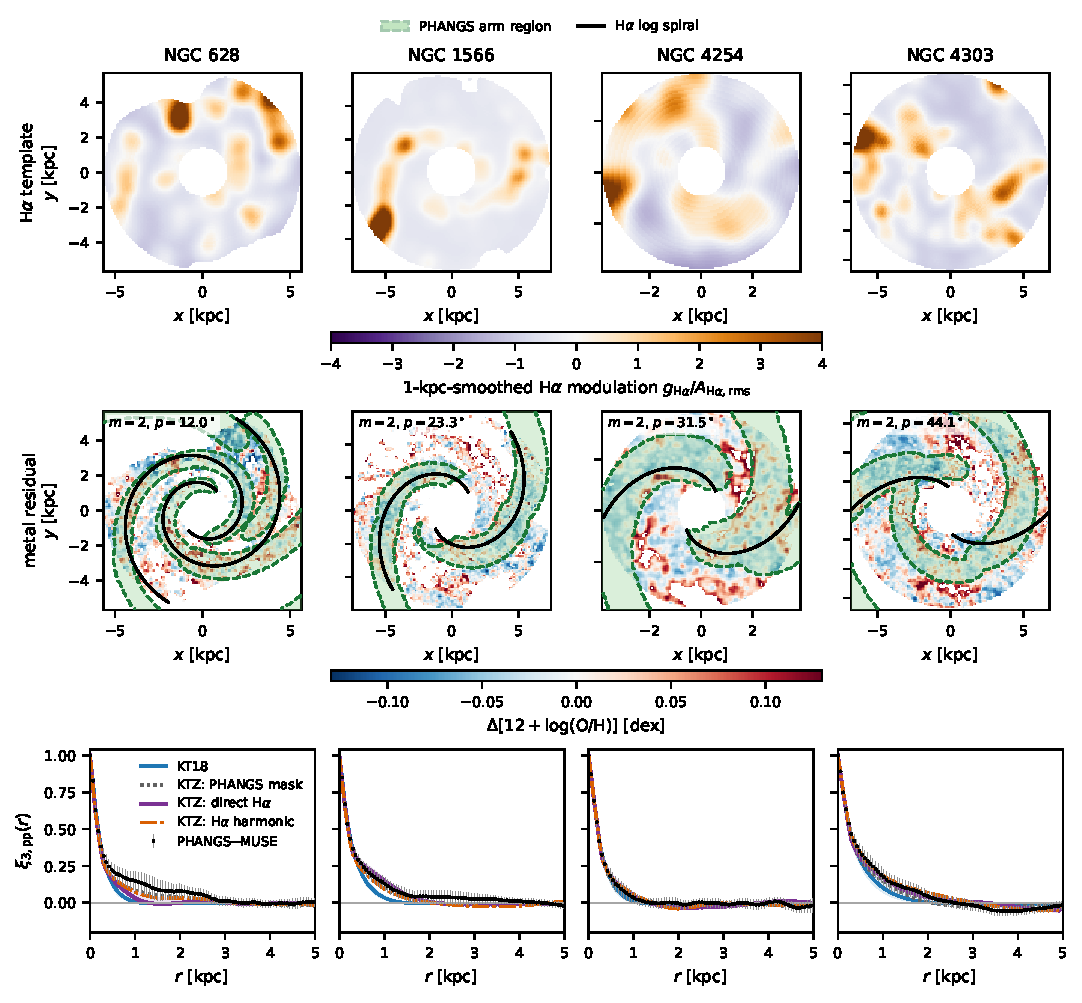
\includegraphics[width=\textwidth]{figs/phangs_four_galaxy_implementation.pdf}
    \caption{Application to the four PHANGS--MUSE galaxies and source-geometry comparison.  Top: the annulus-normalised, 1-kpc-smoothed two-dimensional H$\alpha$ modulation adopted as the primary source template; each map is divided by its rms contrast in Table~\ref{tab:phangs_spirals} for display, but the unscaled map enters the likelihood.  All supported smoothed cells are shown, independently of abundance validity; white unsupported regions are assigned $g_{{\rm H}\alpha}=0$ in the source model.  Middle: oxygen-abundance residual maps used in equation~(\ref{eq:phangs_pair_estimator}); white missing or rejected cells remain \texttt{NaN} and are excluded from the pair statistic.  Green regions with dark-green dashed boundaries show the PHANGS arm-label control, while black solid curves show the H$\alpha$ harmonic geometry.  The abundance window is separate from all source templates, and no source geometry is fitted to the abundance map.  Bottom: measured correlations (points), KT18 (blue), and complete KTZ using the PHANGS mask (grey dotted), direct H$\alpha$ map (purple), or H$\alpha$ harmonic model (orange dash-dotted).  Curves are pointwise posterior medians; bands give the 16th--84th percentiles of KT18 and total direct-H$\alpha$ KTZ.  Error bars use the diagonal of equation~(\ref{eq:phangs_selection_covariance}); fitting uses the full regularised covariance in equation~(\ref{eq:phangs_fit_covariance}).  The $r=0$ point is fixed to unity and is not fitted.}
    \label{fig:phangs_four_galaxies}
\end{figure*}

\subsubsection{Complete KTZ likelihood}
\label{sssec:phangs_inference}

We fit all four terms of the complete KTZ model:
\begin{equation}
    C_{\rm obs}=C_{{\rm 2p},0}+C_{{\rm 2p},N}+C_{\rm M}+C_{\rm NP}.
    \label{eq:phangs_complete_ktz}
\end{equation}
Here $C_{\rm NP}$ is not a post-fit correction.  It is the Gaussian residual source-pair term in equation~(\ref{eq:Esrc_example}), with free ${\cal A}_{\rm src}$ and $\ell_{\rm src}$, and it enters both the numerator and the two endpoint second moments before normalisation.  In accordance with Paper III, it is azimuthally isotropic: its local rate factor is proportional to $\lambda_0^2(R)$ and contains no factor of $g_{{\rm H}\alpha}$, $g_{\rm mask}$, or the harmonic source template.  The deterministic geometry therefore affects only $C_{{\rm 2p},N}$ and $C_{\rm M}$, together with the endpoint moments of those terms.  We do not infer the child fraction and complex multiplicity required to connect this residual covariance uniquely to the harmonic-attenuation formula of a particular Thomas process.  Figure~\ref{fig:phangs_components} shows the resulting four-term model.  Setting $C_{\rm NP}=0$ recovers the conditionally Poisson limit, but that reduced model is not separately fitted or labelled as another version of KTZ here.

For direct comparison with equation~(\ref{eq:phangs_pair_estimator}), the intrinsic model correlation in bin $b$ is
\begin{equation}
    \xi_{{\rm model,int},b}=
    \frac{\displaystyle
    \sum_{(i,j)\in{\cal P}_b}C_{\rm obs}^{(P)}(\bs{x}_i,\bs{x}_j)}
    {\displaystyle\frac{1}{2}
    \sum_{(i,j)\in{\cal P}_b}
    \left[C_{\rm obs}^{(P)}(\bs{x}_i,\bs{x}_i)
    +C_{\rm obs}^{(P)}(\bs{x}_j,\bs{x}_j)\right]}.
    \label{eq:phangs_model_pair_average}
\end{equation}
All retained terms in equation~(\ref{eq:phangs_complete_ktz}) enter this numerator and denominator simultaneously; they are components of one fitted model, not separately fitted curves.

The compressed KTZ calculation returns a finite-window correlation as a function of separation rather than a dense $N_{\rm pix}\times N_{\rm pix}$ covariance matrix.  We therefore implement equation~(\ref{eq:phangs_annular_projector}) as a deterministic response for the stationary-equivalent covariance curve.  We linearly interpolate the model through its zero-lag value and the 83 positive-separation bins, set it to zero beyond 5~kpc, apply $\mathbf P\mathbf C\mathbf P^{\mathsf T}$ on the exact valid-pixel mask, and reduce the result with the same exhaustive estimator.  Because the operation is linear before normalisation, its projected numerator and endpoint-second-moment responses are precomputed once for each covariance coordinate and stored as two $83\times84$ matrices.  Every likelihood evaluation then requires only two matrix products.  This treatment is exact for a separation-only covariance on the adopted mask and is a controlled observing-transfer approximation for the non-axisymmetric KTZ covariance\revdel{; the neglected covariance beyond 5~kpc and the stationary-equivalent reduction are included among the limitations below}.  The same response is applied to KT18.\revadd{  We refer to this calculation as stage 1.  The parameter values reported below come from a second stage that removes the stationary-equivalent reduction and adds an observational nuisance term; stage 1 supplies the abundance map, the covariance, the source template and the starting points of the stage-2 chains.}

\revadd{\paragraph*{Stage 2: exact window projection and pointing zero points.}  For every KTZ component we accumulate the projected numerator and endpoint moments of equation~(\ref{eq:phangs_model_pair_average}) over all $\sim2\times10^7$--$7\times10^7$ pixel pairs on the actual mask, applying $\mathbf P$ to the covariance itself rather than to a separation-only curve.  The same-event terms are accumulated on a kernel-radius grid (10-pc spacing to 0.6~kpc, 60~pc beyond) at five $h_R^{-1}$ nodes and contracted with the KT18 and $C_{\rm NP}$ kernels at likelihood time; the mean-field term is projected as $(\mathbf P\mathbf m)(\mathbf P\mathbf m)^{\sf T}$, which is exact for a deterministic field.  Projecting the pair-averaged $C_{\rm M}(r)$ as if it were stationary double-counts the annular subtraction of an already annulus-normalised mean field; for NGC~4303 the stage-1 treatment overstated the negative wing of $C_{\rm M}$ by a factor of 1.3--2 for all three source geometries.}

\revadd{Each PHANGS--MUSE mosaic is built from 6--12 pointings that were observed, sky-subtracted and flux-calibrated independently.  A constant per-pointing residual $q_p$ in any line that enters the calibration becomes a constant abundance offset over that pointing.  We treat the $q_p$ as unknown nuisance constants with a common Gaussian prior $q_p\sim N(0,\sigma_q^2)$ in units of the residual-field dispersion; marginalising them exactly adds the rank-$K$ covariance $\sigma_q^2\sum_p\mathbf w_p\mathbf w_p^{\sf T}$ with $\mathbf w_p=\mathbf P\mathbf 1_p$, where $\mathbf 1_p$ is the indicator of pointing $p$.  The term is projected through the same operator and the same pair estimator as the physical components, so it is not a free additive curve: its shape is fixed by the mosaic geometry and only $\sigma_q$ is fitted (uniform prior on $[0,3]$).  The pointing footprints are read off the H$\beta$ flux-error plane of the released mosaic, whose noise floor is constant within a pointing and jumps at the seams (\texttt{scripts/phangs\_pointing\_tiles.py}).  To separate $\sigma_q$ from broad physical components, every pixel pair is assigned to a same-pointing or cross-pointing subset and the difference $D(r)=\xi_{\rm same}-\xi_{\rm cross}$, compressed to ten 0.3-kpc bins, is fitted jointly with $\xi_{\rm all}(r)$.  KTZ predicts $D$ only through the exactly projected window difference between the two subsets, which is small and positive, whereas the pointing term enters $D$ directly.  The covariance of the joint vector uses $\boldsymbol\Sigma_{\rm fit}$ for the $\xi_{\rm all}$ block and the 48-block jackknife, with the same shrinkage and floor, for the $D$ block and the cross block; the line-flux Monte Carlo and selection pieces are common to both subsets and cancel in $D$ to first order.  A randomly shifted tiling (60 draws) gives the null distribution of the shoulder-averaged $D$.}

\revadd{Stage 2 also changes two prior choices.  The stage-1 log-normal prior on $\eta$ centred on the tracer contrast is replaced by a flat prior on $\eta$ over the positivity range, so that the arm amplitude is constrained by the abundance statistic alone; and $\ell_{\rm src}$ is bounded below by the 0.12-kpc resolution of the maps, which removes an unresolvable prior-volume mode below the beam.  Sampling uses the same stretch move with 64 walkers and $10^5$ steps (split-$\widehat R\le1.02$), started from the stage-1 posterior.  Bayesian evidences for the nested hierarchy L0 (KT18 transport only), L1 ($+C_{{\rm 2p},N}+C_{\rm M}$), L1n ($+C_{\rm NP}$ only) and L2 (complete KTZ), each with and without the pointing term, are computed with nested sampling \citep[\texttt{dynesty},][]{Speagle2020} on the same joint data vector and priors (400 live points).  Stage 2 is contained in \texttt{NGC$\langle$number$\rangle$\_PHANGS\_\allowbreak exact\_window\_joint.ipynb}, generated by \texttt{scripts/make\_exact\_window\_joint\_notebooks.py}, with the likelihood in \texttt{scripts/ktz\_exact\_window.py} and the evidence in \texttt{scripts/ktz\_exact\_window\_evidence.py}.}

Before MCMC sampling, we visit every unordered observed pixel pair with $r<5$~kpc once.  To reduce memory use without sampling pairs, the code accumulates exact pair counts and the sums of the selected fixed source template $g_{\rm src}$ and $g_{\rm src}^2$ at each pair midpoint, together with the symmetric endpoint sums of $g_{{\rm src},i}+g_{{\rm src},j}$, $g_{{\rm src},i}^2+g_{{\rm src},j}^2$, and $g_{{\rm src},i}g_{{\rm src},j}$.  These quantities are stored in 12 deterministic separation sub-bins within every 0.06-kpc output bin and in 256 midpoint-radius bins.  Each likelihood evaluation combines these precomputed sums with the trial kernel and parameters; it does not revisit the original pixel pairs.  Pair midpoints are evaluated on the 30-pc half-cell grid.  For the two pixel-domain geometries this uses the fixed map directly; only the harmonic control has a Fourier representation and fitted arm locus.  The resulting pair counts agree bin by bin with the independent FFT counts.

We evaluate the transport kernel in the local-source approximation.  The slowly varying radial envelope is evaluated at the pair midpoint; the connected term samples the selected source template at that midpoint, whereas the mean-field endpoint product samples it at both observed cells.  This is a pixel-domain approximation to the general source integral in Paper III, not a new closed analytic solution for an arbitrary measured template.  It is appropriate only when the physical source pattern varies on scales larger than $\ell_\ast$; this motivates smoothing the direct H$\alpha$ map and means that the hard boundary of a released arm label must not be interpreted as resolved physical structure.  The harmonic comparison directly follows the analytic source ansatz.  In all three cases $C_{\rm NP}$ uses only the squared radial rate $\lambda_0^2(R)$ and is independent of the non-axisymmetric template.

The Poisson and mean-field bases are evaluated on an emulator grid with 11 logarithmic nodes in $0.08\leq\ell_\ast/{\rm kpc}\leq3.20$, ten logarithmic nodes in $0.015\leq\epsilon\leq0.90$, and five linear nodes in $-0.35\leq \revdelmath{g_R}\revaddmath{h_R^{-1}}/{\rm kpc}^{-1}\leq0.35$.  The $C_{\rm NP}$ grid adds 17 logarithmic nodes in $0.005\leq\ell_{\rm src}/{\rm kpc}\leq2.50$.  Gaussian quadrature uses 12 nodes for the Poisson/mean-field terms and $14\times14$ age-node pairs for $C_{\rm NP}$.  Re-evaluation with 20 nodes at the primary posterior coordinate medians gives maximum absolute correlation discrepancies of 0.011, 0.021, 0.015, and 0.004 in sample order.  These point checks are not global error bounds and are not added to the likelihood covariance; a precision application requires a denser emulator and validation across posterior support.

The seven fitted coordinates are
\begin{equation}
    \left(
    \ln\ell_\ast,
    \operatorname{logit}\epsilon,
    \ln\beta_{\rm src},
    \ln \revdelmath{s_a}\revaddmath{\eta},
    \revdelmath{g_R}\revaddmath{h_R^{-1}},
    \ln[\beta_{\rm src}{\cal A}_{\rm src}],
    \ln\ell_{\rm src}
    \right).
    \label{eq:phangs_fit_coordinates}
\end{equation}
Here $\ell_\ast$ and $\epsilon$ are the transport scale and dimensionless injection width defined in equation~(\ref{eq:dimensionless_variables}), $\beta_{\rm src}$ is the relative mean-field strength in equation~(\ref{eq:beta_src}), $\revdelmath{s_a}\revaddmath{\eta}$ scales the contrast of the selected fixed source template, and $\revdelmath{g_R}\revaddmath{h_R^{-1}}$ sets the axisymmetric radial rate.  The last two coordinates describe the amplitude and length of residual non-Poisson source clustering.  We sample the product $\beta_{\rm src}{\cal A}_{\rm src}$ because the normalised correlation constrains it more directly than ${\cal A}_{\rm src}$ alone.

This parameterisation follows combinations identifiable from a normalised correlation and prevents the strongly skewed $(\kappa,t_\ast)$ degeneracy from distorting the reported central curve.  We nevertheless define the prior in the physical coordinates used by the model: log-uniform bounds $0.05<\kappa/(\mathrm{kpc^2\,Gyr^{-1}})<1.50$, $0.05<t_\ast/\mathrm{Gyr}<3.00$, $0.015<\sigma/\mathrm{kpc}<0.25$, $10^{-2}<{\cal A}_{\rm src}<10^3$, and $0.005<\ell_{\rm src}/\mathrm{kpc}<2.50$, together with $-0.35<\revdelmath{g_R}\revaddmath{h_R^{-1}}/\mathrm{kpc}^{-1}<0.35$.  These physical bounds are intersected with the emulator domains stated above.  The source scale has $0.10<\revdelmath{s_a}\revaddmath{\eta}<2.50$ and a Gaussian prior in $\ln \revdelmath{s_a}\revaddmath{\eta}$ centred on zero.  Its dispersion is $0.35$ for the direct H$\alpha$ template, encoding tracer-to-enrichment conversion uncertainty; for the mask and harmonic controls it is the larger of 0.35 and the fractional block-bootstrap contrast uncertainty.  Every case is additionally restricted to positive event intensity on the endpoint and midpoint grids.  The prior on $\revdelmath{g_R}\revaddmath{h_R^{-1}}$ is Gaussian with the H$\alpha$ value and uncertainty in Table~\ref{tab:phangs_spirals}.  The exact Jacobian of the transformation to equation~(\ref{eq:phangs_fit_coordinates}) is included.

Converting $\beta_{\rm src}$ into the prior variables $\kappa$ and $t_\ast$ requires a source-rate normalisation.  For this conversion only, we adopt $\mathrm{SFR}=5.5\times10^{-42}L(\mathrm{H}\alpha)$ in $\mathrm{M_\odot\,yr^{-1}}$ \citep{KennicuttEvans2012} and an event-mass distribution $\dd N/\dd M_\ast\propto M_\ast^{-2}$ on $10^2$--$10^6\,\mathrm{M_\odot}$.  The inferred $\kappa$ and $t_\ast$ are therefore conditional on this calibration; the directly constrained combinations $\ell_\ast$, $\epsilon$, and $\beta_{\rm src}$ are the primary reported quantities.

The Gaussian log likelihood is
\begin{equation}
    \ln{\cal L}=-\frac{1}{2}
    \left(\widehat{\boldsymbol\xi}-\boldsymbol\xi_{\rm model}\right)^{\mathsf T}
    \boldsymbol\Sigma_{\rm fit}^{-1}
    \left(\widehat{\boldsymbol\xi}-\boldsymbol\xi_{\rm model}\right)
    +\mathrm{constant}.
    \label{eq:phangs_likelihood}
\end{equation}
We sample it with a Goodman--Weare affine-invariant stretch move \citep{Foreman-Mackey13a}, using 64 walkers and an initial 10,000-step burn-in.  Walkers are initialised from the 64 highest-posterior finite points among 60,000 draws over the bounded physical-prior support, transformed to the coordinates in equation~(\ref{eq:phangs_fit_coordinates}).  Each chain is run for at least 50,000 steps; if the maximum split-$\widehat R$ exceeds 1.05, it is continued in deterministic 25,000-step blocks, up to a pre-declared cap of 150,000 steps.  If slow early settling still leaves $\widehat R>1.05$ at that cap, the burn-in is increased on the same fixed 25,000-step grid and the earliest suffix satisfying the threshold is retained.  For the four primary direct-H$\alpha$ chains, 50,000 steps with the initial burn-in suffice and the maximum split-$\widehat R$ values are 1.016, 1.021, 1.012, and 1.015 in the order of Table~\ref{tab:phangs_sample}.  Every fifth post-burn step is retained for summaries.  We evaluate the deterministic model curve for 1500 samples selected by a separate, galaxy-specific fixed random seed and take its pointwise 16th, 50th, and 84th percentiles.  These intervals propagate posterior parameter uncertainty in the mean correlation but do not include an additional replicated-observation noise draw.  We also fit KT18 independently using the same data, covariance, observing transfer, and marginal transport prior, with 32 walkers, 15,000 steps, and a 4000-step burn-in.  The plotted central curves are pointwise posterior curve medians, not maximum-likelihood curves.

The four primary calculations are contained in \texttt{NGC$\langle$number$\rangle$\_PHANGS\_\allowbreak halpha\_map\_\allowbreak systematic.ipynb}.  The corresponding files with \texttt{fwhm0p5} or \texttt{fwhm1p5} in the name repeat the entire inference at the two bracketing smoothing scales.  The original \texttt{NGC$\langle$number$\rangle$\_PHANGS\_\allowbreak implications.ipynb} notebooks provide the PHANGS-mask controls, and \texttt{NGC$\langle$number$\rangle$\_PHANGS\_\allowbreak logspiral\_systematic.ipynb} provides the continuous-harmonic controls.  \revadd{The stage-2 calculations are \texttt{NGC$\langle$number$\rangle$\_PHANGS\_\allowbreak exact\_window\_joint.ipynb}, which consume the stage-1 products; the H$\beta$-free calibration check is \texttt{scripts/n2s2\_pointing\_check.py} and the stage-2 figure and tables are produced by \texttt{scripts/make\_phangs\_exact\_window\_figure.py}.}  Running any notebook from top to bottom starts from the product identifiers given above and writes the input SHA-256 hashes, nominal and Monte Carlo selections, selection-response and null diagnostics, covariance diagnostics, chains, posterior intervals, residual maps, pair counts, and model curves.

The mask reprojection and H$\alpha$ calibration are implemented in \texttt{scripts/phangs\_environment\_\allowbreak template.py}; the memory-bounded all-pair reduction and source-template KTZ bases are implemented in \texttt{scripts/phangs\_pair\_geometry.py} and \texttt{scripts/phangs\_template\_ktz.py}.  The latter uses only the radial ``uniform'' basis for the unnormalised $C_{\rm NP}$ numerator and endpoint moments, so no source harmonic enters that term; its displayed normalised contribution can still change through the denominator shared with the other components.  The direct-H$\alpha$ notebooks are generated reproducibly by \texttt{scripts/make\_halpha\_map\_\allowbreak systematic\_notebooks.py}, their scale comparison by \texttt{scripts/summarise\_halpha\_\allowbreak smoothing\_sensitivity.py}, and both reported four-galaxy figures by \texttt{scripts/make\_phangs\_four\_\allowbreak galaxy\_figure.py}.  The exploratory H~\textsc{ii}-region and held-out-tail comparisons described below are generated by \texttt{scripts/ktz\_physical\_validation.py}; \texttt{scripts/ktz\_maximum\_\allowbreak likelihood\_diagnostic.py} locates the highest-likelihood retained chain state for the two tail examples.  Neither script defines an additional KTZ observable.

\begin{figure*}
    \centering
    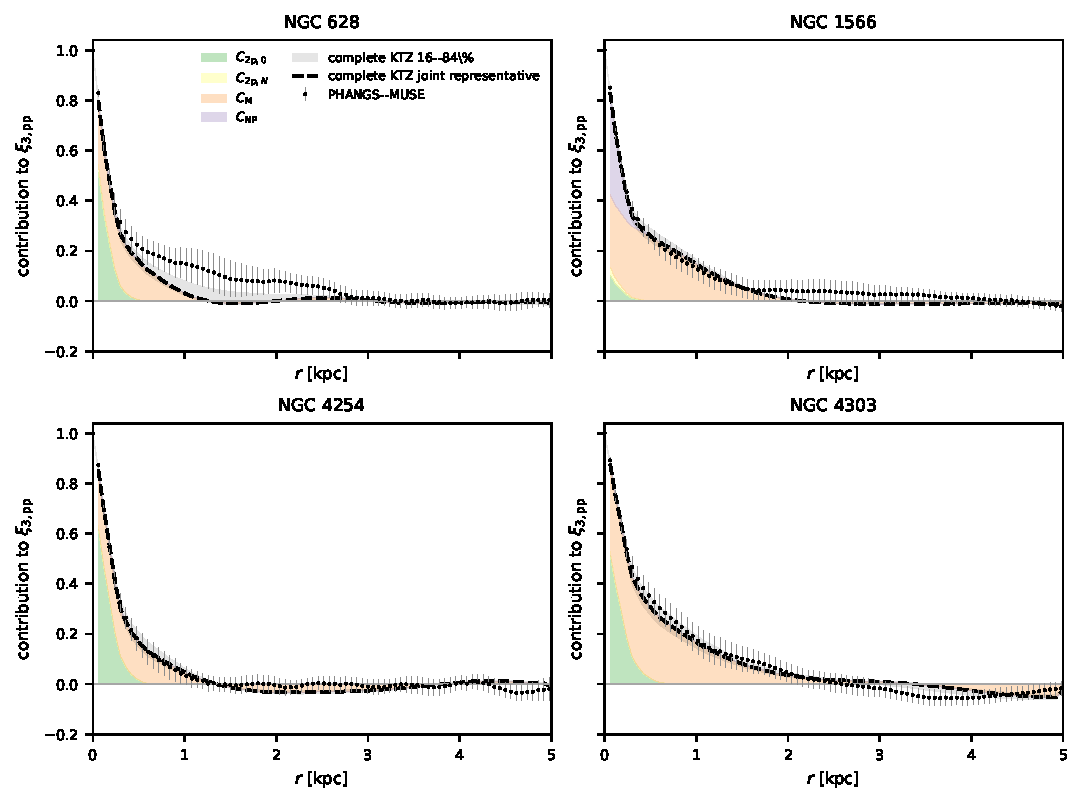
\includegraphics[width=\textwidth]{figs/phangs_four_galaxy_components.pdf}
    \caption{Component decomposition of the complete KTZ fits using the direct two-dimensional H$\alpha$ template.  For each galaxy, we select the joint posterior draw whose total correlation curve is closest to the pointwise posterior-median curve in the fitted covariance metric.  Coloured areas show the cumulative contributions of $C_{{\rm 2p},0}$ (green), $C_{{\rm 2p},N}$ (yellow), $C_{\rm M}$ (orange), and $C_{\rm NP}$ (lavender) from that single draw, after their common annular projection, normalisation, and attenuation by the fixed observing transfer.  The fixed additive correlated measurement-noise bias is omitted from this decomposition.  The black dashed curve is the sum of the four displayed physical components from the same joint draw and therefore coincides with the upper boundary of the stack.  The translucent grey region gives the pointwise 16th--84th percentile interval of the total physical KTZ prediction after subtracting the same fixed noise bias from every posterior draw; individual component intervals are omitted because the components are posterior-correlated and their marginal intervals do not possess a unique additive stack.}
    \label{fig:phangs_components}
\end{figure*}

\subsection{Results and interpretation}
\label{ssec:phangs_results}

Table~\ref{tab:phangs_posteriors} gives the marginal posterior medians and central 68-per-cent intervals for the complete KTZ model.  After applying the same annular projector to every model, we compare its covariance-calibrated discrepancy $\widehat Q$ with the independently fitted KT18 baseline.  This four-object exercise is a morphology and forward-modelling study, not a claim that KTZ is uniformly preferred.  The participation rank of $\boldsymbol\Sigma_{\rm fit}$ is much smaller than the 83 displayed positive-separation bins, which explains why the formerly quoted $Q/(83-p)$ values were much smaller than unity even for two-parameter KT18.  Table~\ref{tab:phangs_posteriors} instead reports equations~(\ref{eq:phangs_fit_covariance}) and (\ref{eq:phangs_calibrated_discrepancy}) for the plotted pointwise posterior-median curves.

\begin{table*}
\centering
\footnotesize
\renewcommand{\arraystretch}{1.3}
\setlength{\tabcolsep}{3.2pt}
\caption{Posterior constraints for complete KTZ using the primary 1-kpc-smoothed two-dimensional H$\alpha$ template.  Entries are marginal medians with 16th--84th percentile offsets.  ${\cal A}_{\rm src}$ and $\ell_{\rm src}$ define the Gaussian residual source-pair excess in equation~(\ref{eq:Esrc_example}).  The final two columns give the covariance-calibrated discrepancy $\widehat Q$ from equation~(\ref{eq:phangs_calibrated_discrepancy}) for the plotted pointwise posterior median KTZ and KT18 curves.}
\label{tab:phangs_posteriors}
\begin{tabular}{@{}lrrrrrrrrr@{}}
\toprule
Galaxy & $\ell_\ast$ [kpc] & $\epsilon$ & $\beta_{\rm src}$ & $\revdelmath{s_a}\revaddmath{\eta}$ & $\revdelmath{g_R}\revaddmath{h_R^{-1}}$ [kpc$^{-1}$] & ${\cal A}_{\rm src}$ & $\ell_{\rm src}$ [kpc] & $\widehat Q_{\rm KTZ}$ & $\widehat Q_{\rm KT18}$\\
\midrule
NGC~628
& $0.150_{-0.022}^{+0.028}$ & $0.232_{-0.096}^{+0.128}$ & $0.802_{-0.346}^{+0.623}$ & $0.966_{-0.220}^{+0.186}$ & $\revdelmath{0.050_{-0.107}^{+0.104}}\revaddmath{-0.050_{-0.104}^{+0.107}}$ & $0.205_{-0.170}^{+1.024}$ & $0.344_{-0.332}^{+1.478}$ & 0.947 & 2.257\\
NGC~1566
& $0.131_{-0.021}^{+0.016}$ & $0.265_{-0.115}^{+0.160}$ & $1.111_{-0.515}^{+0.884}$ & $0.690_{-0.222}^{+0.219}$ & $\revdelmath{-0.194_{-0.029}^{+0.028}}\revaddmath{0.194_{-0.028}^{+0.029}}$ & $45.3_{-44.5}^{+300.9}$ & $0.026_{-0.015}^{+0.062}$ & 0.960 & 1.688\\
NGC~4254
& $0.153_{-0.029}^{+0.034}$ & $0.358_{-0.162}^{+0.221}$ & $3.637_{-2.106}^{+4.571}$ & $0.825_{-0.193}^{+0.202}$ & $\revdelmath{-0.318_{-0.023}^{+0.037}}\revaddmath{0.318_{-0.037}^{+0.023}}$ & $0.337_{-0.310}^{+18.200}$ & $0.029_{-0.020}^{+0.263}$ & 0.712 & 0.456\\
NGC~4303
& $0.163_{-0.036}^{+0.037}$ & $0.266_{-0.135}^{+0.228}$ & $3.197_{-1.894}^{+3.698}$ & $0.699_{-0.166}^{+0.200}$ & $\revdelmath{-0.110_{-0.170}^{+0.205}}\revaddmath{0.110_{-0.205}^{+0.170}}$ & $1.408_{-1.349}^{+61.147}$ & $0.031_{-0.023}^{+0.231}$ & 1.130 & 0.914\\
\bottomrule
\end{tabular}
\end{table*}

\revadd{\begin{table*}
\centering
\scriptsize
\setlength{\tabcolsep}{3.5pt}
\caption{Stage-2 posteriors: exact window projection, flat prior on $\eta$, $\ell_{\rm src}\geq0.12$~kpc, and the pointing zero-point term fitted jointly to $[\xi_{\rm all},D]$.  $\sigma_q$ is in units of the residual dispersion and $f_q$ is the median posterior fraction of the zero-lag residual variance attributed to pointing zero points.  $\chi^2_{\rm joint}$ is the joint discrepancy of the pointwise posterior-median curves (93 data), given for the complete model, for the same model with $\sigma_q\equiv0$, and for the exact-window KT18 reference on $\xi_{\rm all}$ alone (83 data); as in Table~\ref{tab:phangs_posteriors} these are descriptive, because the effective number of covariance modes is 5--13.}
\label{tab:phangs_exact_window}
\begin{tabular}{@{}lccccccccccc@{}}
\toprule
Galaxy & $\ell_\ast$ [kpc] & $\epsilon$ & $\beta_{\rm src}$ & $\eta$ & $h_R^{-1}$ [kpc$^{-1}$] & $\ell_{\rm src}$ [kpc] & $\sigma_q$ & $f_q$ [\%] & $\chi^2_{\rm joint}$ & $\chi^2_{\rm joint}(\sigma_q\!=\!0)$ & $\chi^2_{\rm KT18}$\\
\midrule
NGC~628 & $0.152_{-0.018}^{+0.022}$ & $0.128_{-0.029}^{+0.054}$ & $0.86_{-0.27}^{+0.56}$ & $0.98_{-0.27}^{+0.19}$ & $-0.049_{-0.102}^{+0.105}$ & $0.71_{-0.49}^{+1.10}$ & $0.34_{-0.11}^{+0.08}$ & 4.9 & 10.5 & 14.1 & 28.1\\
NGC~1566 & $0.167_{-0.033}^{+0.040}$ & $0.122_{-0.037}^{+0.074}$ & $2.40_{-1.20}^{+3.12}$ & $0.16_{-0.09}^{+0.11}$ & $0.191_{-0.029}^{+0.029}$ & $0.56_{-0.16}^{+0.18}$ & $0.23_{-0.15}^{+0.13}$ & 2.0 & 4.9 & 5.6 & 19.2\\
NGC~4254 & $0.195_{-0.049}^{+0.069}$ & $0.156_{-0.061}^{+0.101}$ & $7.71_{-4.10}^{+9.00}$ & $0.46_{-0.28}^{+0.33}$ & $0.322_{-0.034}^{+0.020}$ & $0.35_{-0.18}^{+0.24}$ & $0.12_{-0.08}^{+0.10}$ & 0.6 & 7.8 & 7.5 & 7.5\\
NGC~4303 & $0.244_{-0.075}^{+0.115}$ & $0.097_{-0.041}^{+0.084}$ & $10.31_{-6.47}^{+16.47}$ & $0.16_{-0.11}^{+0.18}$ & $0.075_{-0.166}^{+0.153}$ & $0.50_{-0.25}^{+0.19}$ & $0.32_{-0.18}^{+0.15}$ & 3.4 & 10.2 & 11.3 & 9.2\\
\bottomrule
\end{tabular}
\end{table*}}

\revadd{\begin{figure*}
    \centering
    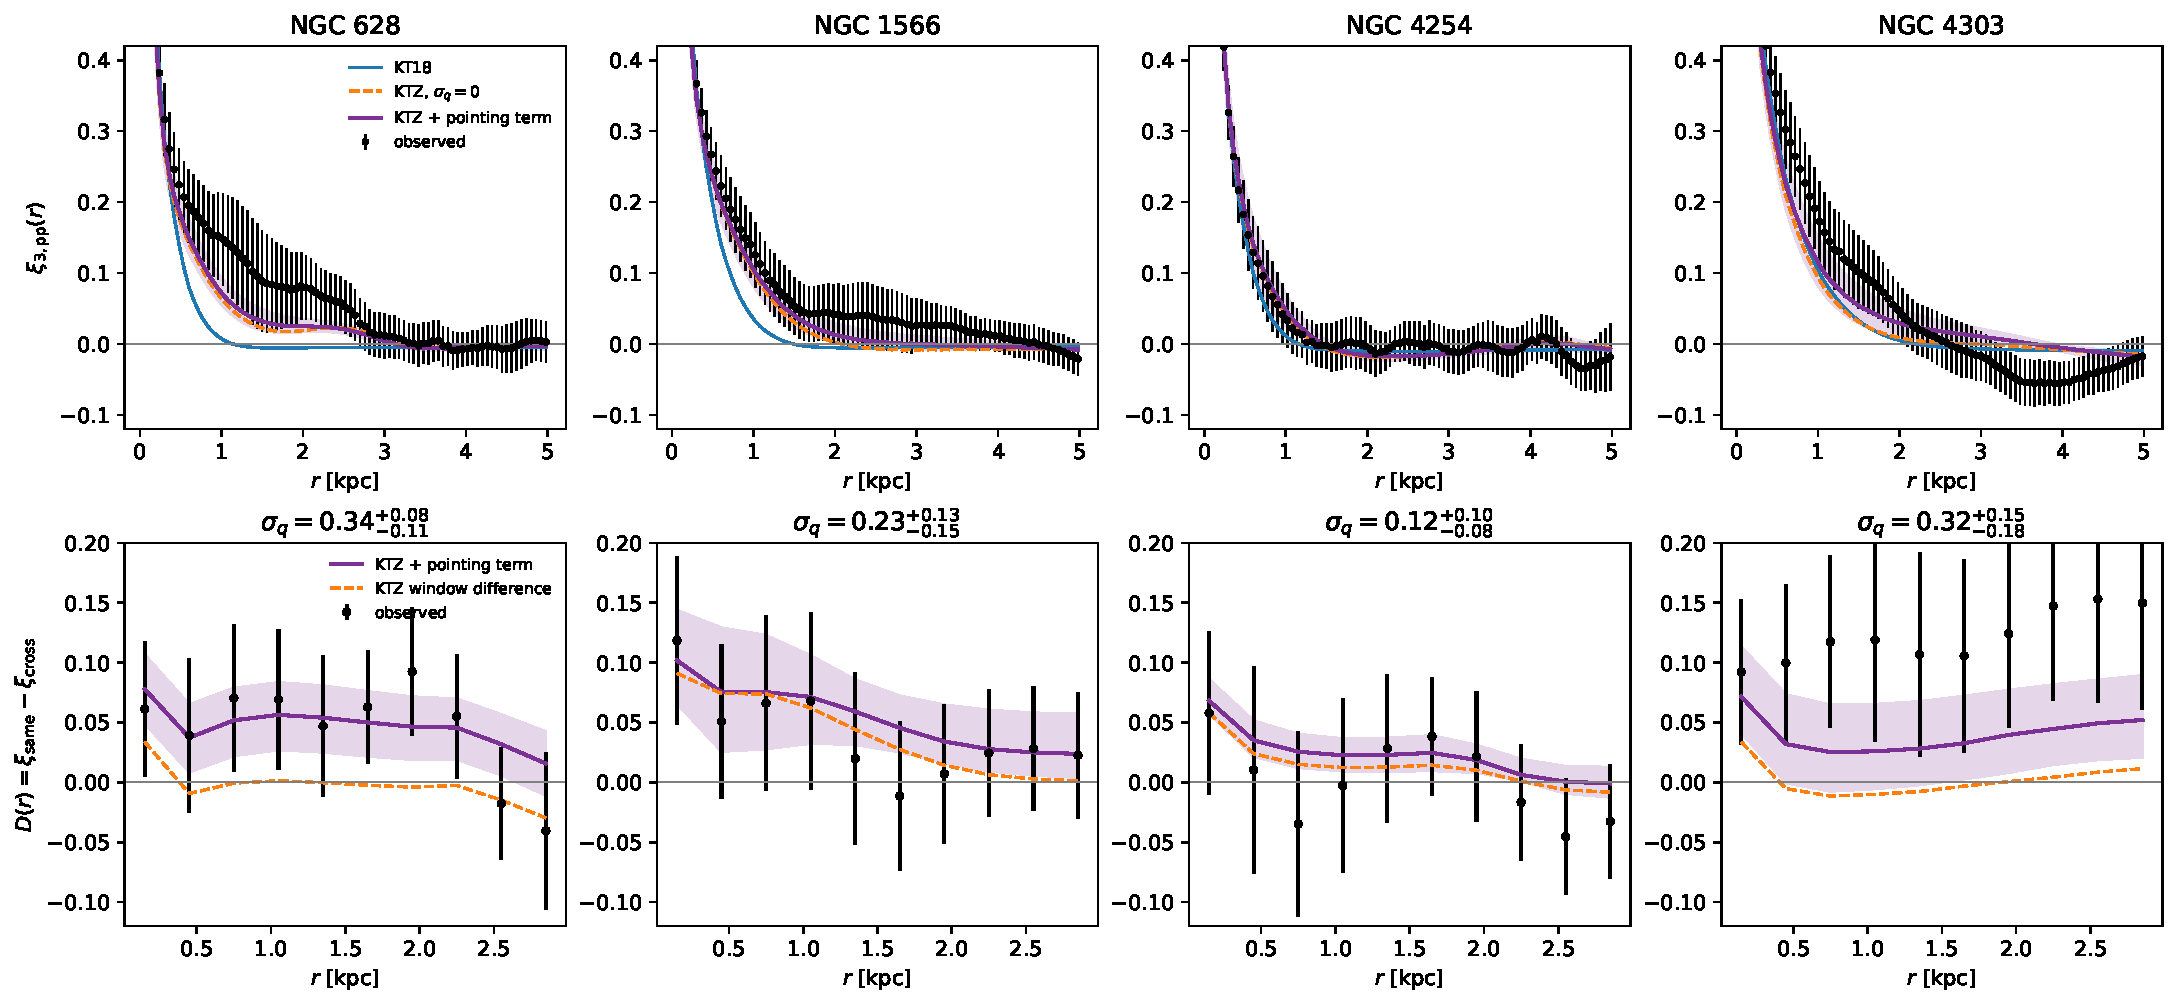
\includegraphics[width=\textwidth]{figs/phangs_four_galaxy_exact_window.pdf}
    \caption{Stage-2 fits.  Top: $\xi_{3,{\rm pp}}(r)$ with the exact-window KT18 reference (blue), complete KTZ without (orange dashed) and with (purple, 16th--84th percentile band) the pointing zero-point term.  Bottom: the same-minus-cross pointing difference $D(r)$ with the KTZ window difference alone (orange dashed) and the complete model (purple); error bars are the jackknife diagonal.}
    \label{fig:phangs_exact_window}
\end{figure*}}

\revadd{\paragraph*{Pointing zero points.}  Splitting the pairs by pointing exposes a systematic that the all-pair statistic cannot isolate.  In NGC~628 and NGC~4303 the shoulder-averaged $D$ exceeds the shifted-tiling null by $z=2.8$ and $z=3.2$ (Fig.~\ref{fig:phangs_exact_window}, bottom), whereas NGC~1566 ($z=1.0$) and NGC~4254 ($z=-0.0$) are consistent with the null.  The fitted amplitudes follow the same ordering: $\sigma_q=0.34^{+0.08}_{-0.11}$, $0.23^{+0.13}_{-0.15}$, $0.12^{+0.10}_{-0.08}$ and $0.32^{+0.15}_{-0.18}$ in the order of Table~\ref{tab:phangs_sample}, i.e.\ a median 5, 2, 1 and 3 per cent of the zero-lag residual variance, or $\simeq0.011$~dex rms per pointing in NGC~628.  Injection tests on the NGC~628 footprint (KT18 fields with and without a mean field, with synthetic per-pointing constants) recover $\sigma_q$ without bias for realised fractions $\geq6$ per cent, produce no false positive at the 0.1--1.5 per cent level, and leave $\ell_\ast$ unbiased when the mean field is present; the two upper limits should therefore be read as $f_q\la4$--5 per cent rather than as measurements.  The term is not interchangeable with $C_{\rm NP}$: it is non-stationary, independent of separation inside a pointing, unfiltered by injection and diffusion, and does not scale with $\lambda_0^2$.  On $\xi_{\rm all}$ alone it is degenerate with a broad, low-amplitude $C_{\rm NP}$; $D(r)$ breaks the degeneracy because $C_{\rm NP}$ treats both pair subsets alike.  Covariance variants (block shape, shrinkage 0.20--0.50, floor 0.005--0.02, a $D$ block from the shifted-tiling null) move $\sigma_q$ within 0.27--0.39 for NGC~628 and 0.24--0.43 for NGC~4303 and $\ell_\ast$ by less than $0.3\sigma$.  We do not subtract fitted per-pointing constants from the map: a least-squares removal absorbs genuine kpc-scale signal and drives the NGC~628 shoulder negative.}

\revadd{The origin of the offsets can be partly localised with the emission lines themselves.  Re-calibrating the identical pixels with the H$\beta$-free N2S2--H$\alpha$ relation of \citet{Dopita2016}, which uses only lines within 170~\AA\ of each other and needs no reddening correction, reduces the edge-aligned excess to $z=1.0$ (NGC~628) and $z=0.7$ (NGC~4303), but that map is 1.5--2 times noisier, and in absolute units the reduction is consistent both with an unchanged and with a removed offset.  More informative are the per-pointing means of the individual line ratios on the same pixels: the per-pointing means of the S-calibration residual correlate with those of $\log([\mathrm{N\,II}]/\mathrm{H}\alpha)$ at $r=0.96$, 0.85, 0.93 and 0.94, but with the Balmer decrement only at $r=0.29$, -0.19, -0.23 and -0.15; and the per-pointing offsets are about twice as large in the fainter half of the H$\alpha$ pixels (rms 0.013/0.027~dex for the S calibration and 0.015/0.029 for $\log[\mathrm{N\,II}]/\mathrm{H}\alpha$ in NGC~628).  The offsets therefore behave as additive per-pointing residuals in the line fluxes -- sky or continuum subtraction differences between observing blocks, which a ratio of adjacent lines does not cancel -- rather than as multiplicative flux-scale or blue-end calibration errors alone.  The statistical treatment does not depend on which line carries the residual.  A direct confirmation requires the per-observing-block cubes, which we have not analysed.}

\revadd{\paragraph*{Exact-window posteriors.}  Table~\ref{tab:phangs_exact_window} and Fig.~\ref{fig:phangs_exact_window} give the stage-2 results.  The transport scale is $\ell_\ast=0.152^{+0.022}_{-0.018}$, $0.167^{+0.040}_{-0.033}$, $0.195^{+0.069}_{-0.049}$ and $0.244^{+0.115}_{-0.075}$~kpc, consistent with stage 1 within the intervals; the exact projection and the pointing term change the curves, not the transport scale.  Under the flat prior the arm amplitude separates the sample: $\eta\simeq1$ in NGC~628, where the smoothed H$\alpha$ contrast is transferred to the abundance field almost unchanged, but $\eta\simeq0.2$--0.5 in the other three, where the stage-1 log-normal prior centred on unity had held it up.  With the resolution bound in place, $\ell_{\rm src}$ is no longer pinned below the beam: $\ell_{\rm src}=0.56^{+0.18}_{-0.16}$, $0.35^{+0.24}_{-0.18}$ and $0.50^{+0.19}_{-0.25}$~kpc for NGC~1566, 4254 and 4303, with the NGC~628 interval still broad ($0.71^{+1.10}_{-0.49}$~kpc).  Whether this component is required is a model-selection question, addressed next.  The exact-window KT18 reference is rejected by the shoulder in NGC~628 and NGC~1566 ($\chi^2=28.1$ and 19.2 for 83 data against 6.0 and 3.6 for the complete model) and is adequate in NGC~4254 and NGC~4303 (7.5 and 9.2 against 5.6 and 7.8).  In NGC~628 the observed shoulder mean over 0.6--2.5~kpc, 0.108, is reproduced as 0.026 from the physical KTZ terms plus 0.022 from the pointing term; the remainder is a 1.4$\sigma$ tension in the covariance metric and the largest residual of the sample.  In NGC~4303 the negative wing at 3--4.5~kpc is not reproduced with the direct H$\alpha$ template under the flat prior (posterior mean $-0.004$ against $-0.049$); with the harmonic template at a 30$^\circ$ pitch it reaches $-0.032$, and the zero crossing of the projected $C_{\rm M}$, which depends on the pitch angle alone (2.35, 2.85 and 3.35~kpc at 25$^\circ$, 32$^\circ$ and 44$^\circ$), matches the observed crossing at 2.7~kpc for $\simeq30^\circ$.  The H$\alpha$ harmonic fit gives $44^\circ$ and the 3.6-$\mu$m two-dimensional Fourier analysis of the S$^4$G image gives $11\fdg3\pm2\fdg4$ over 38--176~arcsec \citep{DiazGarcia2019}; the abundance-implied value lies between the young-star and old-disc pitch angles, and the discrepancy among tracers is the dominant geometric systematic for this strongly barred galaxy.}

\revadd{\paragraph*{Model comparison.}  Table~\ref{tab:phangs_evidence} gives the nested-model evidence on the joint data vector.  The four galaxies do not select the same model.  In NGC~628 the KT18 transport term alone is excluded ($\chi^2_{\min}=34.6$ for 93 data) and the arm-modulated source terms are required, $\Delta\ln Z=+4.6$ for L1 and $+6.3$ with the pointing term; the clustering term adds nothing once the mean field is present.  In NGC~1566 the excluded L0 ($\chi^2_{\min}=19.4$) is repaired by the isotropic clustering term instead ($\Delta\ln Z=+1.0$, $\chi^2_{\min}=6.5$), and the arm terms are penalised ($-0.5$).  In NGC~4254 and NGC~4303 L0 is adequate ($\chi^2_{\min}=10.3$ and 12.2) and carries the highest evidence; the additional KTZ components are tolerated, not required.  The transport scale depends on the model family: under L0 alone it is $\ell_\ast\simeq0.37$--0.68~kpc, whereas every model that includes a kpc-scale component returns 0.15--0.25~kpc, because the shoulder that a broad component absorbs would otherwise have to be carried by a wider kernel.  The statement that $\ell_\ast$ is universally small is therefore a statement within the KTZ family, established where that family is required (NGC~628, NGC~1566) and assumed elsewhere.  A compact prior on the clustering amplitude changes the evidences by less than 1.5~nat and none of the orderings.}

\revadd{\begin{table}
\centering
\scriptsize
\setlength{\tabcolsep}{2.5pt}
\caption{Nested-model evidence on the joint $[\xi_{\rm all},D]$ vector (stage-2 priors).  $\Delta\ln Z$ is relative to L0 (KT18 transport only); suffix q adds the pointing term.  Errors on $\ln Z$ are 0.1--0.2.}
\label{tab:phangs_evidence}
\begin{tabular}{@{}lrrrrrrrr@{}}
\toprule
Galaxy & L0 & L0q & L1 & L1q & L1n & L1nq & L2 & L2q\\
\midrule
NGC~628 & $+0.0$ & $+0.8$ & $+4.6$ & $+6.3$ & $+4.6$ & $+3.1$ & $+4.6$ & $+4.1$\\
NGC~1566 & $+0.0$ & $-0.8$ & $-0.5$ & $-2.5$ & $+1.0$ & $+0.2$ & $-1.0$ & $-2.7$\\
NGC~4254 & $+0.0$ & $-2.5$ & $-3.1$ & $-5.8$ & $-2.0$ & $-4.7$ & $-5.6$ & $-8.1$\\
NGC~4303 & $+0.0$ & $-1.5$ & $-5.1$ & $-6.2$ & $-2.1$ & $-3.5$ & $-7.6$ & $-9.0$\\
\midrule
$\chi^2_{\min}$ NGC~628 & 34.6 & 28.7 & 13.3 & 9.7 & 16.2 & 16.1 & 11.8 & 9.5\\
$\chi^2_{\min}$ NGC~1566 & 19.4 & 16.7 & 11.0 & 10.9 & 6.5 & 4.3 & 4.9 & 4.3\\
$\chi^2_{\min}$ NGC~4254 & 10.3 & 10.3 & 8.7 & 8.7 & 7.1 & 7.1 & 6.7 & 7.0\\
$\chi^2_{\min}$ NGC~4303 & 12.2 & 11.1 & 12.0 & 10.7 & 10.4 & 8.9 & 10.3 & 8.6\\
\bottomrule
\end{tabular}
\end{table}}

\revadd{The stage-1 decomposition is retained below because the controls (mask, harmonic, smoothing) were run in that framework.}  The component decomposition shows that the inferred allocation between coherent source structure and residual source association is geometry-dependent.  With the primary 1-kpc-smoothed H$\alpha$ template, the four posteriors do not establish a resolved $C_{\rm NP}$ scale.  NGC~1566 has a formally large ${\cal A}_{\rm src}=45.3^{+300.9}_{-44.5}$ but a compact $\ell_{\rm src}=0.026^{+0.062}_{-0.015}$~kpc, well below the 120-pc beam; the two parameters are strongly degenerate and do not constitute a measured cloud scale.  NGC~4254 and NGC~4303 show the same compact-boundary behaviour with long upper tails.  NGC~628 permits a broader scale, but its interval extends from $0.012$ to $1.82$~kpc and its amplitude is likewise weakly identified.

At $r=0.48$~kpc, the direct-H$\alpha$ posterior-median $C_{\rm NP}$ contributions to the observed normalised statistic are only 0.007, 0.003, 0.005, and 0.009 for NGC~628, NGC~1566, NGC~4254, and NGC~4303, respectively.  The corresponding $C_{\rm M}$ contributions are 0.130, 0.260, 0.159, and 0.291.  By contrast, the PHANGS-mask control assigns broad intermediate-scale contributions to $C_{\rm NP}$ in NGC~628 and NGC~1566 because its binary arm regions do not encode the observed within-arm H$\alpha$ intensity structure.  The direct template transfers much of that power into the deterministic mean-field term.  This comparison is evidence of a decomposition systematic, not evidence that non-Poisson clustering vanishes: ${\cal A}_{\rm src}$ has a strictly positive log prior, unresolved source non-stationarity and observing covariance can project onto the same component, and no nested $C_{\rm NP}=0$ calculation has been used for model selection.  A detection claim would require that the inferred component persist under pre-specified source templates and smoothing scales and be favoured in a calibrated nested comparison.

NGC~4303 provides a useful posterior-predictive limitation.  The annular projector can produce a negative wing, but the strength of that wing depends on the source geometry and on the stationary-equivalent projection approximation.  Forcing the curve through the pointwise tail by changing its weights or adding an unconstrained negative offset would not be justified; a stronger claim requires a better calibrated covariance and a full non-stationary implementation of equation~(\ref{eq:phangs_annular_projector}).

KTZ is sensitive to the source geometry even after the two-dimensional covariance is reduced to an angle-averaged function of separation.  The geometry enters $C_{{\rm 2p},N}$ through the source rate at each pair midpoint and enters $C_{\rm M}$ through products of the convolved mean field at the two endpoints.  It also affects the endpoint second moments that normalise equation~(\ref{eq:phangs_model_pair_average}).  By construction, $C_{\rm NP}$ does not depend on the non-axisymmetric template.  The finite footprint and annular projector assign different weights to the remaining geometric contributions, so templates with similar global contrast but different phase, pitch, width, or branching can produce different shoulders and negative wings in $\xi_{3,{\rm pp}}(r)$; a radial average does not necessarily erase this dependence.

Figure~\ref{fig:phangs_four_galaxies} quantifies this effect while leaving the seven-dimensional likelihood unchanged.  The values of $\widehat Q$ for the PHANGS mask, direct H$\alpha$ map, and H$\alpha$ harmonic geometry are respectively $(0.708,0.947,0.612)$ for NGC~628, $(0.790,0.960,1.285)$ for NGC~1566, $(0.735,0.712,0.709)$ for NGC~4254, and $(1.264,1.130,0.709)$ for NGC~4303.  Their mixed ordering is evidence for a morphology systematic rather than a uniform gain from greater template detail.  For NGC~4303 specifically, the posterior-median mean over $3.3\leq r/{\rm kpc}\leq4.5$ is $-0.019$, $-0.025$, and $-0.038$ for the same three geometries, compared with the observed $-0.049$; the covariance-weighted training-only check below tests whether this remains true when the tail is excluded.  The change is driven mainly by the deterministic mean-field geometry rather than by an independently added negative component.  H$\alpha$ traces recent massive-star formation and is physically closer to prompt oxygen injection, whereas the broad 3.6-$\mu\mathrm{m}$/CO-defined PHANGS masks retain non-logarithmic branches and may better describe the longer-lived structural environment.  The harmonic compression can preserve a coherent large-scale phase while discarding local irregularities.  No representation is universally preferable; the direct H$\alpha$ map is the declared primary prompt-enrichment input, and the other two expose its morphology dependence.  A larger-sample inference should place externally calibrated uncertainty on source geometry and marginalise over it jointly with the transport parameters.

The additional low-pass scale is a modelling systematic, not an observational resolution.  Table~\ref{tab:phangs_halpha_smoothing} reports the pre-specified 0.5/1.0/1.5-kpc comparison; we do not select its smallest discrepancy as the final template.  Across the converged runs, the median $\ell_\ast$ ranges from 0.115 to 0.172~kpc in NGC~628, 0.124 to 0.173~kpc in NGC~4254, and 0.116 to 0.171~kpc in NGC~4303.  The NGC~4303 tail remains less negative than observed at every scale.  NGC~628 additionally changes from a broad $\ell_{\rm src}\simeq1.65$~kpc at 0.5-kpc smoothing to a compact, weakly identified source-pair term at 1.5-kpc smoothing.  Thus the division between $C_{\rm M}$ and $C_{\rm NP}$ cannot yet be regarded as template-robust.  The NGC~1566 1.5-kpc chain reaches the declared 150,000-step cap with $\max\widehat R=1.072$, principally in the two source-pair coordinates; its numerical products are retained with a convergence flag but excluded from the formal comparison.

\begin{table*}
\centering
\small
\caption{Sensitivity to the pre-specified direct-H$\alpha$ smoothing FWHM $w$.  The first three columns give the covariance-calibrated discrepancy of the pointwise posterior-median curve, and the last three give its arithmetic mean over $3.3\leq r/{\rm kpc}\leq4.5$.  A dash excludes the NGC~1566 1.5-kpc chain that failed the $\widehat R\leq1.05$ convergence rule.  The metallicity map, observing transfer, priors, and seven likelihood coordinates are otherwise unchanged.}
\label{tab:phangs_halpha_smoothing}
\begin{tabular}{@{}lrrrrrr@{}}
\toprule
 & \multicolumn{3}{c}{$\widehat Q$ at $w$ [kpc]} & \multicolumn{3}{c}{$\overline\xi_{3.3\text{--}4.5}$ at $w$ [kpc]}\\
Galaxy & 0.5 & 1.0 & 1.5 & 0.5 & 1.0 & 1.5\\
\midrule
NGC~628  & 0.681 & 0.947 & 0.931 & $-0.012$ & $-0.005$ & $-0.006$\\
NGC~1566 & 0.673 & 0.960 & --    & $-0.006$ & $-0.010$ & --\\
NGC~4254 & 0.693 & 0.712 & 0.791 & $ 0.002$ & $ 0.000$ & $-0.008$\\
NGC~4303 & 1.182 & 1.130 & 1.227 & $-0.015$ & $-0.025$ & $-0.024$\\
\bottomrule
\end{tabular}
\end{table*}

Although the direct H$\alpha$ template never uses abundance residual values, it is not an independent data set: it shares emission-line noise, attenuation correction, and star-forming selection with the abundance map.  Mask-aware smoothing does not reconstruct emission in genuinely unobserved regions, nor does instantaneous H$\alpha$ uniquely specify the source history over $t_\ast$.  The external PHANGS-mask control and the smoothing comparison therefore remain necessary, and source-template uncertainty is not included in the conditional posterior bands of Fig.~\ref{fig:phangs_four_galaxies}.

To distinguish a posterior-volume effect from a limitation of the source representation, we also examine the highest-likelihood retained states of the mask and harmonic controls for NGC~1566 and NGC~4303 after subtracting the analytic prior from the saved posterior log density.  This is a diagnostic within the sampled physical support, not a replacement for the posterior summaries.  In particular, a visually improved harmonic tail obtained only when $\revdelmath{g_R}\revaddmath{h_R^{-1}}$ approaches a prior boundary is evidence of parameter sensitivity rather than a stable measurement of the radial source profile.

A single maximum-likelihood curve also does not account for the five additional KTZ coordinates relative to KT18.  As an indicative, rather than definitive, complexity check, $\mathrm{AIC}=\chi^2_{\rm ML}+2p$ gives 20.23 and 22.72 for the NGC~1566 PHANGS-mask KTZ and KT18 fits, respectively, but 18.51 and 12.88 for the NGC~4303 H$\alpha$-geometry KTZ and KT18 fits.  The former difference is weak and the latter favours the simpler model despite the more accurate KTZ tail mean.  These values should not be promoted to a formal selection result because the likelihood contains strongly correlated modes and the KTZ analysis uses informative external priors.  They show why we retain posterior-predictive curves and held-out tests as the main evidence, and use the maximum-likelihood state only to establish whether a feature lies within the model family.

The positivity limits implied by the primary direct-H$\alpha$ templates are $\revdelmath{s_a}\revaddmath{\eta}<1.250$, $1.036$, $1.201$, and $1.053$ for NGC~628, NGC~1566, NGC~4254, and NGC~4303, respectively; none of the reported central intervals is forced against these limits.  One radial boundary effect remains important: for NGC~4254 the direct H$\alpha$ estimate $\revdelmath{g_{R,\mathrm{H}\alpha}=-0.378}\revaddmath{h_{R,{\rm H}\alpha}^{-1}=0.378}\pm0.056$~kpc$^{-1}$ lies just outside the adopted emulator range, and the fitted $\revdelmath{g_R}\revaddmath{h_R^{-1}}$ posterior approaches its \revdel{lower}\revadd{upper} boundary at $\revdelmath{-0.35}\revaddmath{0.35}$~kpc$^{-1}$.  Its radial-rate and non-Poisson constraints should consequently not be interpreted independently of this bound.  More generally, this four-galaxy application demonstrates that the KTZ terms can be mapped onto resolved data without assigning the arm signal to the metallicity field itself, but it is not a population-level test: abundance calibration, finite-window geometry, the local-source approximation for measured templates, \revdel{the stationary-equivalent annular response and its 5-kpc covariance truncation}\revadd{the pointing footprints read off the noise floor and the independence of the per-pointing constants}, and the assumed isotropic Gaussian form of residual source clustering remain shared modelling choices.\revadd{  The stage-1 covariance is conservative: all four stage-2 $\chi^2$ values are well below the number of data, so shape tensions such as the NGC~1566 outer plateau and the NGC~4303 wing may be larger than the $\chi^2$ suggests; and $t_\ast$ sits at its 0.05-Gyr prior bound in three galaxies, so $\kappa$ and $t_\ast$ separately are calibration-conditional.}

\subsubsection{Fixed-radius correlations}
\label{sssec:phangs_xi2_results}

The exhaustive $\xi_{2,{\rm pp}}(R_m,r)$ calculation contains 22,086,188, 43,047,620, 18,443,424, and 67,351,964 unordered pairs for NGC~628, NGC~1566, NGC~4254, and NGC~4303, respectively.  It shows substantial radial variation: the inner NGC~1566 and NGC~4303 intervals turn negative at smaller separation than their outer intervals, whereas the outer NGC~628 correlation remains positive across the evaluated range.  This confirms that $\xi_{3,{\rm pp}}(r)$ compresses distinct radial behaviours.  We do not further divide these pairs by a binary arm/interarm classification.  Such a division is not part of the KTZ derivation and discards the continuous harmonic amplitude and phase information that distinguishes the source models.

\subsection{Exploratory external comparisons}
\label{ssec:phangs_physical_checks}

The component labels become physically informative only if quantities inferred from the metal correlation agree with observables that were not constructed from the metal residual field.  We therefore perform two deliberately separate checks.  First, we test whether the scale ordering inferred for ${\cal A}_{\rm src}$ and $\ell_{\rm src}$ is present in the spatial point process of current star-forming regions.  We select PHANGS catalogue H~\textsc{ii} regions with \texttt{FLAG\_EDGE=FLAG\_STAR=0}, \texttt{BPT\_NII=0}, positive finite attenuation-corrected H$\alpha$ luminosity, and $0.1\leq R/R_{25}\leq0.4$.  For each galaxy we draw a random catalogue eight times larger than the data catalogue from the 60-pc source window with probability density
\begin{equation}
    p_{\rm ran}(\bs{x})\propto
    \exp[\revdelmath{g_{R,{\rm H}\alpha}(R-R_{\rm ref})}\revaddmath{-(R-R_{\rm ref})/h_{R,{\rm H}\alpha}}]
    [1+g_{\rm mask}(\bs{x})].
    \label{eq:phangs_hii_random_intensity}
\end{equation}
Thus the null catalogue contains the independently measured radial gradient, footprint, arm widths, branches, and H$\alpha$-calibrated arm contrast, but not residual clustering below that template.  With $DD$, $DR$, and $RR$ denoting pair counts normalised by the corresponding total possible numbers of pairs, we estimate the remaining excess using
\begin{equation}
    \widehat{\mathcal E}_{\rm HII}(r)
    =\frac{DD(r)-2DR(r)+RR(r)}{RR(r)}
    \label{eq:phangs_hii_landy_szalay}
\end{equation}
\citep{LandySzalay1993}.  Errors and parameter intervals use a delete-one-sector jackknife with 12 equal azimuthal sectors.  The PHANGS segmentation and deblending suppress distinct catalogue centroids in the first $0$--$0.12$~kpc bin; we display neither that bin nor use it in the fit.  Over $0.18\leq r/{\rm kpc}\leq2.46$, we fit the same latent Gaussian form as equation~(\ref{eq:Esrc_example}), ${\cal A}_{\rm HII}\exp[-r^2/(2\ell_{\rm HII}^2)]$.  This source-catalogue fit is not included in the metallicity likelihood.

\begin{table*}
\centering
\scriptsize
\setlength{\tabcolsep}{5pt}
\caption{Independent source-pair check conditioned on the PHANGS-mask control.  The H~\textsc{ii}-region entries are Gaussian fits to equation~(\ref{eq:phangs_hii_landy_szalay}), with 12-sector jackknife intervals.  The KTZ entries repeat the mask-control metal-correlation posterior constraints for the latent source-pair excess, because the same externally defined intensity is required in the random catalogue.  The two estimators probe different source selections, so agreement in ordering is more robust than equality of their amplitudes.}
\label{tab:phangs_hii_source_pairs}
\begin{tabular}{@{}lrrrrr@{}}
\toprule
Galaxy & $N_{\rm HII}$ & ${\cal A}_{\rm HII}$ & $\ell_{\rm HII}$ [kpc] & ${\cal A}_{\rm src}$ & $\ell_{\rm src}$ [kpc]\\
\midrule
NGC~628  & 2059 & $0.105_{-0.014}^{+0.016}$ & $1.216_{-0.096}^{+0.104}$ & $0.293_{-0.170}^{+0.317}$ & $1.499_{-0.763}^{+0.584}$\\
NGC~1566 & 1179 & $0.254_{-0.025}^{+0.028}$ & $0.794_{-0.084}^{+0.094}$ & $0.558_{-0.224}^{+0.257}$ & $0.520_{-0.087}^{+0.101}$\\
NGC~4254 &  832 & $0.150_{-0.012}^{+0.013}$ & $0.504_{-0.124}^{+0.164}$ & $0.135_{-0.110}^{+3.879}$ & $0.042_{-0.033}^{+0.389}$\\
NGC~4303 & 1676 & $0.172_{-0.023}^{+0.027}$ & $0.715_{-0.159}^{+0.205}$ & $0.109_{-0.086}^{+1.056}$ & $0.123_{-0.113}^{+0.729}$\\
\bottomrule
\end{tabular}
\end{table*}

The upper four panels of Fig.~\ref{fig:phangs_physical_validation} compare the residual H~\textsc{ii}-region pair excess with the $C_{\rm NP}$ scale inferred in the PHANGS-mask control.  We deliberately do not condition the random catalogue on the direct H$\alpha$ template, because using the same current H~\textsc{ii} emission both as the null intensity and as the point catalogue would weaken the independence of the check.  Similar scale ordering would be physically suggestive because the H~\textsc{ii} positions are measured without using the metal residual values, but it would not establish that the two quantities trace the same point process.  The comparison is not statistically independent of abundance selection: both the nebular catalogue and the valid-spaxel mask favour line-bright star-forming regions.  The ratio-shuffle null constrains the resulting selection-induced metal correlation in the released-map pipeline, but it cannot reproduce every native-cube detection and segmentation effect.  We therefore treat the four-object ordering as descriptive only, and do not expect equality of the numerical scales: H~\textsc{ii} centroids are a luminosity-selected, deblended snapshot, whereas ${\cal E}_{\rm src}$ describes a latent enrichment-event process integrated over the KTZ source-age window.

Our second check asks whether the NGC~4303 negative wing can be predicted rather than fitted.  We remove all $r\geq3$~kpc bins from the likelihood, retain the same priors and covariance model, and use the converged full-range chain only as an importance-sampling proposal.  If $\boldsymbol\theta_i$ is a saved draw, its training-only weight is
\begin{equation}
    w_i\propto
    \frac{{\cal L}_{r<3\,{\rm kpc}}(\boldsymbol\theta_i)}
         {{\cal L}_{r<5\,{\rm kpc}}(\boldsymbol\theta_i)}.
    \label{eq:phangs_tail_importance_weight}
\end{equation}
The training likelihood uses the corresponding covariance submatrix, so correlations among retained bins are preserved.  The effective importance-sample sizes are 4266, 2896, and 7068 for the PHANGS-mask, direct-H$\alpha$, and H$\alpha$-harmonic KTZ proposals, respectively, and 35,955 for KT18; these values indicate that the reweighting is not dominated by a few draws, although a dedicated training-only chain would be a stronger support check.  Over the held-out interval $3.3\leq r/{\rm kpc}\leq4.5$, the observed arithmetic mean is $-0.049$.  The training-only predictions are $-0.021^{+0.005}_{-0.004}$, $-0.026^{+0.008}_{-0.012}$, and $-0.037^{+0.013}_{-0.020}$ for the same three KTZ geometries, and $-0.011^{+0.003}_{-0.002}$ for KT18.  Only the harmonic-template interval contains the observed tail mean.  However, the tail-submatrix quadratic residuals of their pointwise median curves are 2.52, 5.19, 3.47, and 3.58, respectively.  Thus the improved harmonic tail mean is not a uniform improvement in the covariance-weighted detailed tail shape.

\begin{figure*}
    \centering
    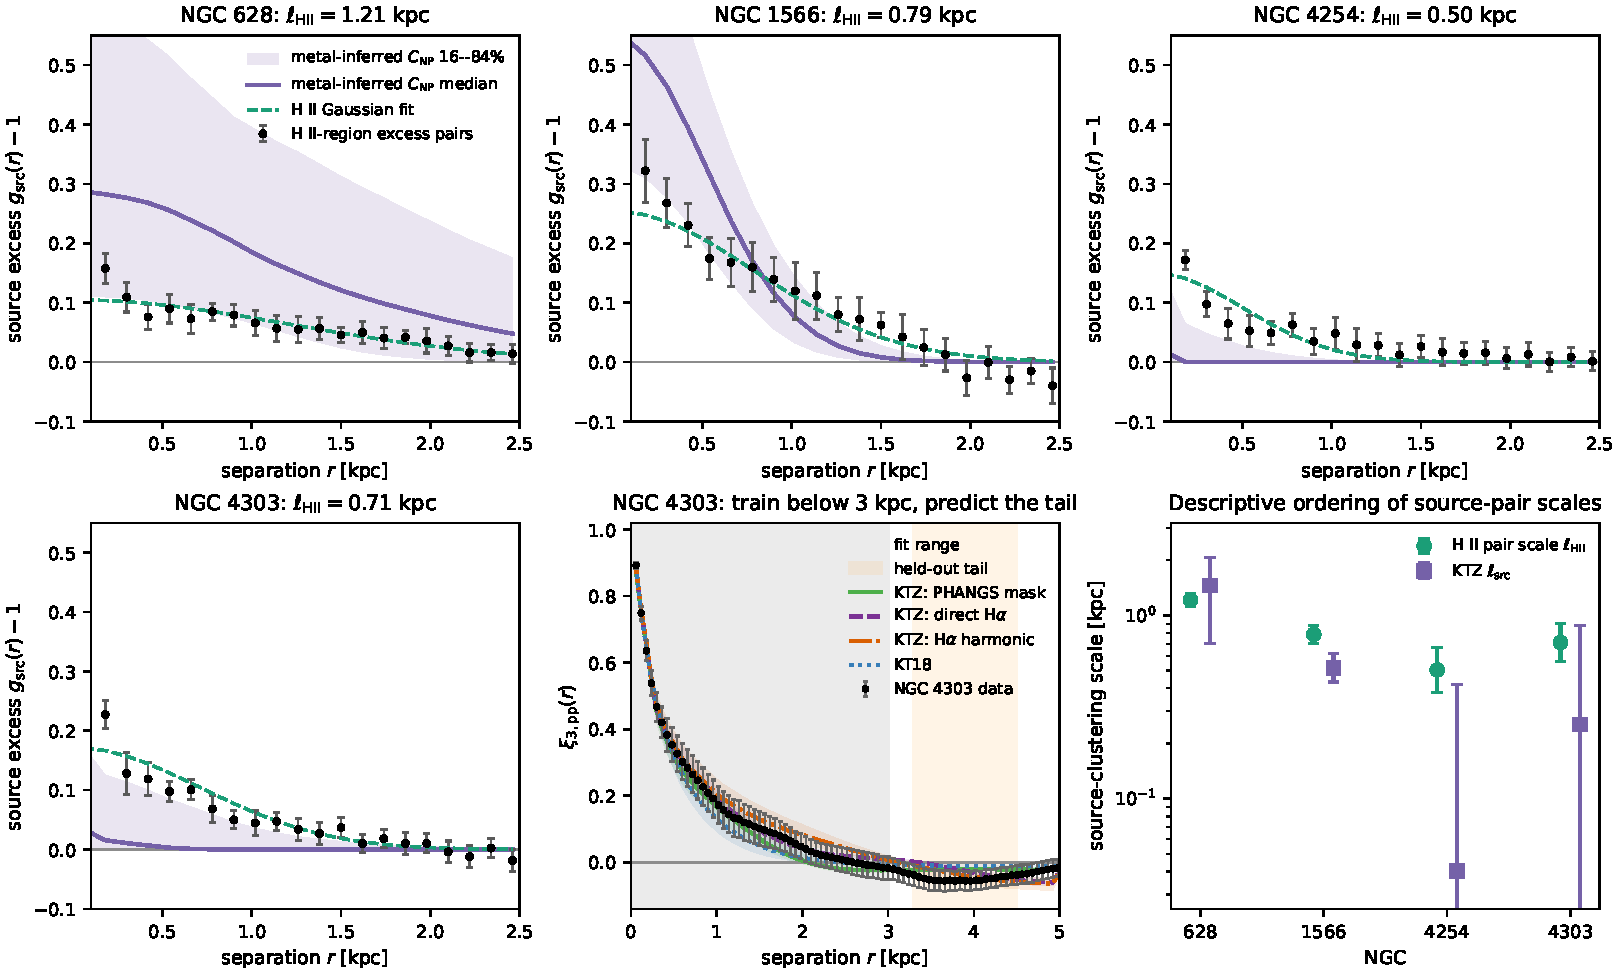
\includegraphics[width=\textwidth]{figs/phangs_ktz_physical_validation.pdf}
    \caption{Exploratory external comparisons for complete KTZ.  The first four panels compare the residual pair correlation of qualified PHANGS H~\textsc{ii}-region centroids (points) with a Gaussian fit to those points (green dashed) and the latent source-pair excess inferred from the PHANGS-mask metallicity fit (lavender).  The omitted $0$--$0.12$~kpc catalogue bin is affected by segmentation/deblending.  The lower-middle panel compares all three source geometries in the NGC~4303 experiment: only the grey $r<3$~kpc interval enters the likelihood, while the orange $3.3$--$4.5$~kpc tail is predicted.  Bands give pointwise 16th--84th percentiles.  The lower-right panel compares the independently fitted and mask-control metal-inferred source-clustering scales; the common rank ordering is descriptive for four objects and does not persist as a resolved constraint in the primary direct-H$\alpha$ decomposition.}
    \label{fig:phangs_physical_validation}
\end{figure*}

The held-out calculation illustrates how an independently measured source geometry can alter a large-scale prediction that is not used to constrain the transport coordinates, whereas uniform KT18 has no corresponding morphology input.  It is not a confirmatory prediction: the H$\alpha$ logarithmic spiral was examined after the NGC~4303 wing was noticed, and the detailed covariance-weighted tail shape is not uniformly improved.  A blind test would have to pre-register the source tracer, geometry algorithm, and held-out statistic on a larger sample.  Here the calculation is retained only as an exploratory sensitivity test.


\section{Discussion}
\label{sec:discussion}

\subsection{Interpretation of the development sample}
\label{ssec:discussion_development}

KTZ is not an unconstrained family of correlation curves: its large-scale shape is inherited from a two-dimensional source model and from the observing operation applied to that model.  A practical application should therefore proceed in two stages.  The source tracer, spatial filtering, and geometry representation should first be declared without reference to the metal residual correlation.  A pixel-domain representation fixes the entire measured field and requires no arm number or pitch angle; a harmonic representation instead fixes the arm number, pitch, phase, width, and coefficients, and hence $k_\perp(\varpi)$, from an independent tracer such as H$\alpha$, ultraviolet emission, CO, or a near-infrared stellar-structure map.  The abundance statistic can then constrain the reduced transport coordinates $(\ell_\ast,\epsilon)$, the conversion between tracer and enrichment-event contrast, and the relative stochastic and mean-field amplitudes.  In particular, when harmonics are used, $q_n=nk_\perp\ell_\ast$ is derived from the constrained morphology and trial transport scale; treating it as an additional independent fitting coordinate would erase the physical connection that KTZ is intended to test.

The separation of terms also identifies what an observed tail can constrain.  At $r\gg\ell_\ast$, the uniform same-event contribution $C_{{\rm 2p},0}$ and its local rate-modulation correction $C_{{\rm 2p},N}$ are strongly suppressed.  The remaining shape is governed mainly by the deterministic mean-field term $C_{\rm M}$ and any broad different-event term $C_{\rm NP}$ after the finite footprint, pair average, and radial-profile subtraction have been applied.  The first of these can be positive or negative because pairs at a specified separation sample different phases of the convolved source pattern.  The adopted $C_{\rm NP}$ is a single-scale positive Gaussian excess before the observing transfer, but annular mean subtraction can give its projected contribution a compensating negative lobe.  Consequently, neither the sign nor the node of the measured tail is controlled by a free additive offset.  A negative wing is primarily a test of coherent source geometry and its phase relative to the footprint, whereas a positive shoulder can constrain residual source association only over the scales on which it is statistically resolved.

The two most visually distinctive PHANGS cases illustrate this distinction.  In NGC~1566, the measured mean over $3.3\leq r/{\rm kpc}\leq4.5$ is $0.013\pm0.015$; it is therefore consistent with zero once the fitted bin covariance is retained.  The posterior-median predictions from the three source representations remain slightly negative, between $-0.021$ and $-0.011$.  This is not evidence that a significant positive tail lies outside KTZ.  Rather, the likelihood is constrained mainly by the resolved $0.3$--$1$~kpc shoulder: extending the single Gaussian $C_{\rm NP}$ sufficiently to raise the outer bins also raises the better-constrained intermediate bins and is partly cancelled by the annular projector.  Establishing a distinct positive tail would require either more independent large-separation modes or a pre-specified, physically motivated multi-scale source-pair model.

For NGC~4303, by contrast, the sign is accessible to KTZ but its amplitude depends strongly on the externally supplied morphology.  The PHANGS arm-region and direct-H$\alpha$ templates predict training-only tail means of $-0.021^{+0.005}_{-0.004}$ and $-0.026^{+0.008}_{-0.012}$, respectively, compared with the observed $-0.049$.  The independently measured H$\alpha$ harmonic geometry gives $-0.037^{+0.013}_{-0.020}$ and contains the observed mean even when the tail is excluded from the fit; its best-likelihood full-range curve reaches $-0.038$.  Thus the model family can produce most of the negative wing through deterministic geometry, but the primary direct map does not recover its full amplitude.  The greater coherence of the harmonic compression is a plausible explanation, not an identified cause\revdel{, because the non-axisymmetric annular projection is approximate}\revadd{.  With the exact projection of stage 2 the wing predicted by every template is smaller than in stage 1, and under the flat $\eta$ prior the direct template no longer produces it, so the wing is evidence about the pitch angle of the enriching pattern ($\simeq30^\circ$ from the $C_{\rm M}$ zero crossing) rather than about transport}.  This result is a proof of principle, not a detection of a unique geometry: the harmonic alternative was examined after the wing was noticed, its best fit is sensitive to the allowed radial-rate boundary, and its detailed covariance-weighted tail shape is not uniformly superior.  A decisive test should fix the source tracer and morphology prescription before examining the metal correlation and repeat the held-out prediction over a larger sample.

These examples also show why a maximum-likelihood curve should be used diagnostically rather than as the primary observational summary.  It establishes whether a feature is reachable within the parameterised model, but it neither represents posterior uncertainty nor penalises the five additional KTZ coordinates relative to KT18.  Moreover, the 83 plotted separation bins correspond to only about 5--13 effective covariance modes in the present maps.  The pointwise posterior median and posterior-predictive interval are therefore more stable summaries than a single optimum, while the covariance-calibrated discrepancy and held-out predictions are more meaningful than a nominal reduced $\chi^2$ constructed by treating every plotted bin as independent.

Map construction must be included in the forward model.  Here the 60-pc cell size is a sampling interval, whereas 0.2~kpc is the width of the annuli used to estimate the axisymmetric abundance profile; it is not a pixel scale.  The same annular projector and exact valid-pixel footprint are applied to KTZ and KT18, and rejected cells remain \texttt{NaN} rather than being filled with zero.  The dynamic-threshold and line-ratio-shuffle experiments show that ordinary selection-boundary crossings are much too small to generate the measured shoulders and tails.  The larger changes obtained under deliberately different line and equivalent-width cuts nevertheless show that sample definition is a genuine systematic.  Future applications should therefore report sensitivity to annulus width and abundance-pixel selection, including an H~\textsc{ii}-segmentation-only comparison, and should use native-cube injection and recovery where the data permit it.

The H~\textsc{ii}-region comparison supplies a preliminary external consistency check on the PHANGS-mask $C_{\rm NP}$ interpretation.  Its similar scale ordering is compatible with an origin in organised recent star formation, but the direct-H$\alpha$ and smoothing comparisons show that this ordering is not a template-robust metal constraint.  There are only four objects, the abundance and nebular samples share line-bright selection, and an isotropic Gaussian term can absorb unmodelled non-stationarity or observing covariance.  A physical inference requires a nested no-$C_{\rm NP}$ comparison, posterior-predictive checks under alternative abundance calibrations and source templates, and source-pair priors measured independently from H~\textsc{ii} regions, clusters, or molecular clouds.

Cross-element applications should use the same externally constrained morphology with the channel transfers ${\cal J}_{0,ab}^{AB}$ and ${\cal J}_{n,ab}^{AB}$; mean-field terms are retained unless the maps have been explicitly de-spiralled.  If residual source clustering is required, the non-zero azimuthal harmonics should be fixed or marginalised jointly with the isotropic distinct-event extension derived in Paper III, because a complete azimuthal average discards their phase distinction.  Paper III summarises the combinations accessible to normalised statistics and the external information required to separate their dimensional factors.  In this form, the observational value of KTZ is not that it must outperform KT18 for every galaxy, but that it connects departures from a uniform correlation curve to independently measurable source geometry, source association, and element-dependent transport.

\subsection{Scope of the geometry comparison}
\label{ssec:geometry_scope}

The present observable is the angle-averaged pair-product statistic.  Its dependence on source morphology arises because the finite footprint and radial-profile projector do not weight every midpoint and orientation equally, and because $C_{\rm M}$ retains products of the continuously convolved source field.  This establishes a controlled comparison between three externally specified source representations, but it is not a direct measurement of arm/interarm chemical contrast or of phase locking.  In particular, neither rotating a source mask nor thresholding a harmonic template into ``rich'' and ``poor'' regions follows from the current KTZ derivation.

A future phase-resolved test should first be derived in the same continuous language as the theory.  A natural observable is the complex Fourier coefficient of the residual pair product at fixed midpoint radius and separation.  Its modulus and argument can then be compared with the amplitude attenuation and phase shift predicted for the corresponding externally measured source harmonic, after applying the identical PSF, selection, annular projection, and finite window.  Until that statistic and its covariance have been derived and validated numerically, the present four-galaxy analysis supports only a morphology-sensitivity statement based on $\xi_{2,{\rm pp}}$ and $\xi_{3,{\rm pp}}$; it does not constitute a phase-resolved validation of KTZ.

\section{Conclusions}

We have constructed a reproducible application of complete KTZ, including isotropic $C_{\rm NP}$, to four PHANGS--MUSE spiral galaxies.  The emission-line data, abundance selection, finite footprint, radial-profile subtraction, beam, and correlated measurement response are carried through the same exhaustive pair estimator used for the model.  The direct two-dimensional H$\alpha$ field, PHANGS arm-region mask, and continuous H$\alpha$ harmonic model are treated as three representations of the same source-intensity input and are never used to divide the metallicity pairs into binary arm and interarm samples.

\revadd{A second inference stage projects every KTZ component exactly through the annular-mean operator on the actual mask and marginalises an observational nuisance: independent zero points of the MUSE pointings, constrained by the same-minus-cross pair difference $D(r)$.  Such zero points are detected in NGC~628 and NGC~4303 (3--4 per cent and 5 per cent of the residual variance, $\simeq0.01$~dex rms) and bounded in NGC~1566 and NGC~4254; they trace additive per-pointing line-flux residuals rather than the H$\beta$ calibration alone.  With the exact projection, a flat prior on the arm amplitude and a resolution bound on $\ell_{\rm src}$, the transport scale is $\ell_\ast=0.15$--0.25~kpc in all four galaxies.  Nested-model evidence shows that KT18 transport alone is excluded in NGC~628 and NGC~1566 and repaired by different KTZ components -- the arm mean field in the former, isotropic source clustering in the latter -- while NGC~4254 and NGC~4303 are consistent with KT18; within KT18 alone $\ell_\ast$ would be 0.4--0.7~kpc, so the small transport scale is a result within the KTZ family.}  The present angle-averaged fits do not show that KTZ is uniformly preferred to KT18.  In NGC~4303 both the PHANGS arm-region and primary direct-H$\alpha$ templates underpredict the negative tail, whereas an independently fitted H$\alpha$ harmonic model predicts most of its mean amplitude even when the tail is excluded from the likelihood.  Because that alternative geometry was examined after the feature was noticed and because the best fit is sensitive to the radial-rate boundary, it remains a development-sample demonstration rather than a confirmatory detection.  The weak positive outer mean in NGC~1566 is statistically consistent with zero.

The pre-specified 0.5/1.0/1.5-kpc H$\alpha$ smoothing comparison changes the inferred transport scale and allocation between $C_{\rm M}$ and $C_{\rm NP}$ appreciably.  In particular, the broad source-pair structure inferred with the binary arm masks is not recovered as a robust resolved component with the primary direct template.  Conditional posterior bands therefore understate uncertainty if the source representation is treated as exact; a physical source-clustering claim requires template and observing-transfer systematics to be marginalised or independently constrained.

The fixed-radius calculation reveals strong radial variation in $\xi_{2,{\rm pp}}$, but no phase statistic is inferred from a thresholded source map.  A genuine phase-resolved test requires the continuous complex harmonic observable and observing-window response to be derived and validated first.  The present results therefore establish the feasibility of applying the KTZ pair-product formalism and quantify its sensitivity to externally specified morphology; they do not constitute a phase-resolved or population-level validation of non-uniform injection.

\section*{Acknowledgements}

\section*{Data Availability}

\bibliographystyle{mnras}
\bibliography{example}

%%%%%%%%%%%%%%%%%%%%%%%%%%%%%%%%%%%%%%%%%%%%%%%%%%

% Don't change these lines
\bsp
\label{lastpage}
\end{document}
